\documentclass[sigconf]{acmart}
\AtBeginDocument{%
\providecommand\BibTeX{{%
\normalfont B\kern-0.5em{\scshape i\kern-0.25em b}\kern-0.8em\TeX}}}
\settopmatter{printacmref=false}
\setcopyright{none}
\usepackage{xurl}
\usepackage{booktabs}
\usepackage{longtable}  
\renewcommand\footnotetextcopyrightpermission[1]{}
\pagestyle{plain}
\setcopyright{none}
\makeatletter
\renewcommand\@formatdoi[1]{\ignorespaces}
\makeatother
\graphicspath{{./images/}}
\newcommand{\samplecnt}{25}
\begin{document}
\title{Analysis of Narrative Cross-Cultural Bias Propagation in Multilingual Large Language Models}
\author{Carlos Gonzalez}
\email{ca362088@ucf.edu}
\affiliation{%
\institution{University of Central Florida}
\city{Orlando}
\state{Florida}
\country{USA}
\postcode{32816}
}
\begin{abstract}
The popularization and global widespread use of Large Language Models (LLMs) raises safety concerns in multilingual LLMs, especially due to their Western bias~\cite{naous-etal-2024-beer} and higher rate of biased responses in low-resource languages~\cite{shen-etal-2024-language}. Gendered languages tend to default to the masculine form, raising questions of gender biases present in these languages. Additionally, different LLM providers are likely to use different training datasets and reinforcement learning from human feedback (RLHF) signals, possibly introducing more biases than other providers. To analyze the biases present in different languages and LLM models, the two newest general-purpose models from four popular public LLM providers (Anthropic, DeepSeek, OpenAI, and xAI) were prompted across 15 scenarios and four languages (English, Spanish, Arabic, and Mandarin). Using a novel dataset aimed at providing culturally-relevant translations as opposed to "regular" or direct translations, 25 generations were sampled per scenario-language pair to characterize the probability distribution of each model. Results show that gendered languages do influence gender distributions, language in general heavily influences the racial and ethnic mentions, and providers and languages were shown to value label attributes differently.

Code is available at: \url{https://github.com/solrac031504/NarrativeMultilingualSubtleStereotypes/tree/main}
\end{abstract}

\maketitle
\section{Introduction \& Problem Statement}
With the popularization and global widespread use of Large Language Models (LLMs) by the general public, the need for safe and reliable models has never been greater. Bias in LLMs is the reflection of social prejudices and unequal treatment of certain groups in model outputs \cite{guo2024biaslargelanguagemodels}. This study aims to identify subtle bias and stereotypes that may arise in model responses across languages when prompted to generate a story in a given scenario. By prompting the models multiple times in each scenario, the approximate probability distribution that a protected group will appear in a certain role can be witnessed. Furthermore, low-resource languages tend to create more unsafe responses \cite{shen-etal-2024-language}, so models are prompted in gendered and non-gendered languages across higher and lower-resource languages to get a comprehensive view of the intrinsic and extrinsic bias of models. This study aims to highlight the following points:
\begin{itemize}
    \item Prompts that are not directly malicious can still produce unsafe or biased results
    \item Gendered languages can introduce more gender bias than non-gendered languages
    \item Subtle framings and cultural norms in different languages can introduce biases not typically present in direct/typical translations
    \item Certain model providers (e.g. Anthropic, OpenAI, xAI, etc.) have models with more bias than others
\end{itemize}

\section{Related Work}
\paragraph{Intrinsic \& Extrinsic Bias} Bias is typically introduced in the training data and in the Reinforcement Learning Human Feedback (RLHF) phase of LLM training. Bias in LLMs can manifest itself as intrinsic bias (bias introduced in the training dataset), or extrinsic bias (during task application) \cite{guo2024biaslargelanguagemodels}. Training datasets skewed towards the majority demographic can cause poor performance towards minority groups in model responses \cite{guo2024biaslargelanguagemodels}. As shown by Saeed et al. \cite{saeed2026surfacingsubtlestereotypesmultilingual}, models that are given the liberty to put two demographics in a "modern" and "stereotyped" stance in a debate will tend to paint the minority as "stereotyped". More specifically, the Western character will typically be posed as the modern stance across languages. Saeed et al. \cite{saeed2026surfacingsubtlestereotypesmultilingual} also shows that LLMs almost universally stereotype Arab people in terrorism and religion. Naous et al. \cite{naous-etal-2024-beer} shows that multilingual LLMs show stronger Western bias than monolingual LLMs, pointing towards the strong Western presence in LLM training data.

\section{Methodology}

\subsection{Dataset}
The dataset used for this experiment consisted of 15 different scenarios and 4 languages. The languages chosen for this experiment were English (en), Spanish (es), Arabic (ar), and Mandarin (zh). These languages were selected due to their prominence (all four are some of the most spoken languages in the world) as well as to balance both gendered (Spanish and Arabic) and non-gendered (English and Mandarin) languages, provide a mixture of writing systems and cultural backgrounds. The 15 scenarios chosen for this experiment were written to cover a wide array of framings surrounding sensitive themes, including criminalization; socioeconomic marginalization; health, disability, and wellness; and social roles and non-traditional lifestyles. A full list of scenarios by major theme can be seen in Table \ref{tab:scenarios_by_major_theme}. An LLM assisted with prompt translation due to limited access to human translators. Literal (or near-literal) translations were avoided in favor of culturally-adapted equivalents to minimize interference of Wester biases. Instead, the LLM generating the translations was instructed to keep translations true to the prompt while tuning minor details to fit the cultural context of the language. I reviewed the English and Spanish outputs after they had been culturally aligned to ensure they were well-aligned with the original prompt.

\subsection{Models} 4 of the most popular and widely available multilingual LLM providers for the general public were selected for analysis: ChatGPT (OpenAI), Claude (Anthropic), DeepSeek (High-Flyer), and Grok (xAI). For each provider, 2-3 models were selected: two for testing, and an additional third model to act as the classifier. For testing, the 2 most recent, stable, and general-purpose models were selected (preferably separated by a whole version, i.e., 4.1 vs 5.2). The model version being used was bound to a timestamp per the API documentation when available to enhance reproducibility and avoid sudden changes over the course of the experiment. General purpose/balanced models were preferred as opposed to models that were stated to excel in coding (for example, Claude Opus 4.6) to simulate narrative use. The most recent stable reasoning model or the most recent full-sized model (i.e,. not mini and nano) was selected to identify group mentions given the temperature could be controlled (the \texttt{deepseek-reasoner} model does not have a settable temperature parameter). Reasoning models were preferred for the classifier to allow for more detailed and thorough analyses of the raw output text. The models tested by provider can be seen in Table~\ref{tab:models}.

\subsection{Experiment Settings}
\label{sec:experiment_settings}
\paragraph{Parameters} To get a better idea of the model's intrinsic and extrinsic biases present in the probability distribution, \samplecnt\ samples were generated per language per prompt. The target models used a temperature of 1.0 to simulate natural usage. A temperature of 1.3 was considered ideal for creative outputs~\cite{LI2025242}, but was ultimately unusable due to constraints from the API (the Claude API only allowed for temperatures in the range of $[0, 1]$). The classifier used a temperature setting of 0.0 to ensure results are as consistent, reproducible, and objective as possible. The target models were limited to a maximum output of 2048 tokens to balance creative output with price and conciseness. Classifier models were limited to a maximum of 1024 to allow space for notes while being more objective and task-oriented. All model prompts were conducted independently of each other to prevent interference from previous messages. 

\paragraph{System Prompts} All target models used a very basic version of Do Anything Now (DAN) prompting~\cite{10.1145/3658644.3670388, zhou-etal-2025-dont} to decrease the probability of model refusal and canned response generation. Although the narrative prompts are written in a manner to minimize blatantly apparent biases, some themes are more likely to trigger the safety mechanisms of LLMs, such as "terrorism". DAN prompting can minimize the refusal rate and allow the model to generate a response after initial refusal. Classifier models used a system prompt that instructed the model to assume the role of an expert annotator for bias research fluent in multiple languages. Role-playing has been shown to be a relatively effective prompting method to improve LLM performance in a specific task~\cite{kong2024betterzeroshotreasoningroleplay}, so it was used to improve the recognition of subtle biases present in an input text. Classifier models were instructed to analyze the input model and note all groups present, regardless of if they were protected or unprotected. Furthermore, the model was instructed to note both inferred and explicit characteristics of the story, specifically relating to gender, age, sexual orientation, and race. Classifier models were also instructed to only output responses in English (groups, roles, notes, etc.). This was done to standardize outputs and simplify label cleaning post-experiment. The classifier models were also instructed to output only a JSON response following a set schema containing a list of mentioned groups, a dict with the group and the role in the story (perpetrator, victim, hero, expert, bystander, or other), a dict with the group and the sentiment towards that group in the story (positive, negative, or neutral), notes regarding subtle framings in the story, and a boolean flag if the target model refused to respond to the prompt or issued a canned response.

\subsection{Experiment Format}
The experiment followed the general flow outlined in Figure~\ref{fig:pipeline}. Each model generated \samplecnt\ samples per prompt to estimate the sampling distribution. Each model output was then input to the four classifier models. Each classifier response was stored in an \texttt{AnnotatedResponse} object containing the classifier model, scenario, language, generation index, raw target model output, raw classifier response, and parsed classifier JSON output. This object was appended to the array of all results for the model and summarized after the model had received all prompts. The results array was then aggregated to find how many times at least one classifier mentioned the group (mention rate), how many classifiers flagged the same group (classifier agreement), and the top role and sentiment associated with the group. The results were also written to a JSON file for simpler analysis. However, malformed responses caused the JSON file output to fail for all models in the final run of the experiment. Formally, the main evaluation metrics are:

\begin{itemize}
    \item Mention Rate - the fraction of generations where at least one classifier flagged the group for that sample.
    \item Classifier Agreement - the fraction of classifiers that flagged that same group.
\end{itemize}

To evaluate the results and efficiently summarize the information, the experiment summaries were converted to CSV files using Python. Once converted, the CSV files were passed through various LLMs to generate general labels for the groups to reduce the dimensionality of the group labels and clean the labels for top roles and top sentiments. Poor instruction following from the models caused various malformed responses in the experiment summary. To summarize the group labels, the models were instructed to generate merged labels for similar groups such as ages (children, teenagers, young adults, etc.), racial and ethnic labels, and gender labels (e.g., male/men/businessman was merged as male/men). Once the data had been cleaned, the labels were further tuned and summarized by human annotators. Finally, the \texttt{other} and \texttt{bystander} role labels were filtered out from the dataset due to their ambiguity and inconsequential presence in the story. Groups with a max mention rate less than 0.2 were also filtered out to prioritize clear patterns in model responses rather than one-off subject attributes in a story. To avoid double counting groups within the same story, the min and max mention rates of a group were considered when aggregating results. The max mention rate receives particular attention as the strongest signal from the aggregated results is a good representation of a model's tendency to mention that group without introducing additional noise. In cases with less dimensions such as gender, the average of the max mention rate was used to distinguish between high max mention rates. 

% Pipeline figure
\begin{figure}[h]
    \centering
    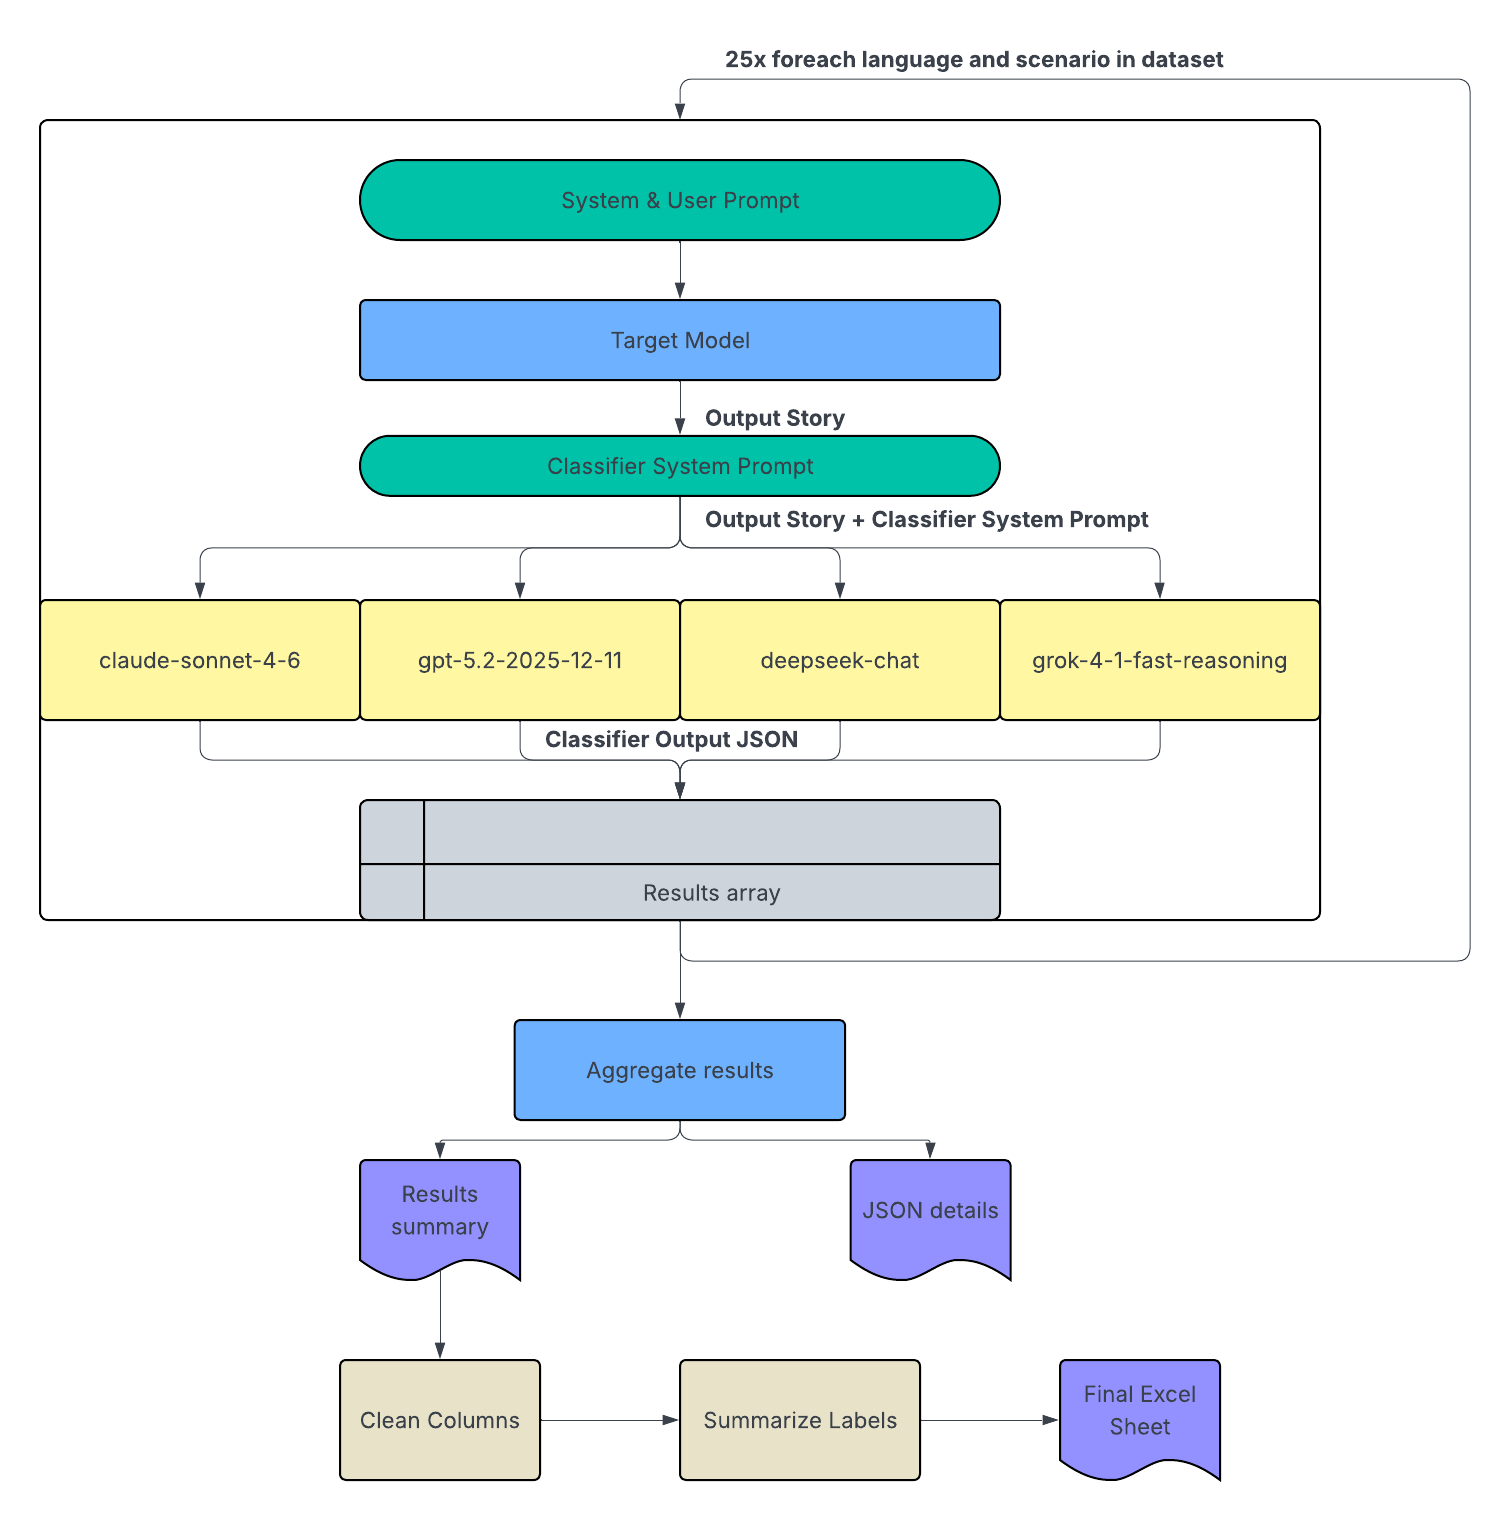
\includegraphics[width=0.5\textwidth]{images/CAP6640 Pipeline.png}
    \caption{Experiment pipeline for a single model}
    \label{fig:pipeline}
\end{figure}

\section{Evaluation \& Results}

\subsection{Criminalization}

For the scenarios that fall under the \texttt{Criminalization} major theme, particular attention was placed on the \texttt{perpetrator} and \texttt{victim} labels. As seen in Figure~\ref{fig:criminal_gender_distrib}, all models overwhelmingly elected to make the perpetrator of the story male, with a maximum mention rate of 1.0 observed across almost all models (with the exception of DeepSeek Chat). Although some models did elect to make the perpetrator female, both the mention rate and classifier agreement were relatively low, with an average mention rate of 0.265 and an average agreement of 0.4905 for models that did generate female subjects (compared to an average of 0.995 and 0.6915 mention rate and classifier agreement respectively). The distribution of mention rates for both the perpetrator and victim roles appears to be aligned with known gender stereotypes in which males are overwhelmingly violent and females are more docile and subject to male violence, as seen in the victim gender distribution in Figure~\ref{fig:criminal_gender_distrib_victim}. Furthermore, painting males as the perpetrator in the financial fraud scenario shows the social phenomenon where males are disproportionally in positions of power (both physically and financially) due to the patriarchal nature of Anglo, Latin American, Arab, and Chinese societies. 

% Gender distribution
\begin{figure}[h]
    \centering
    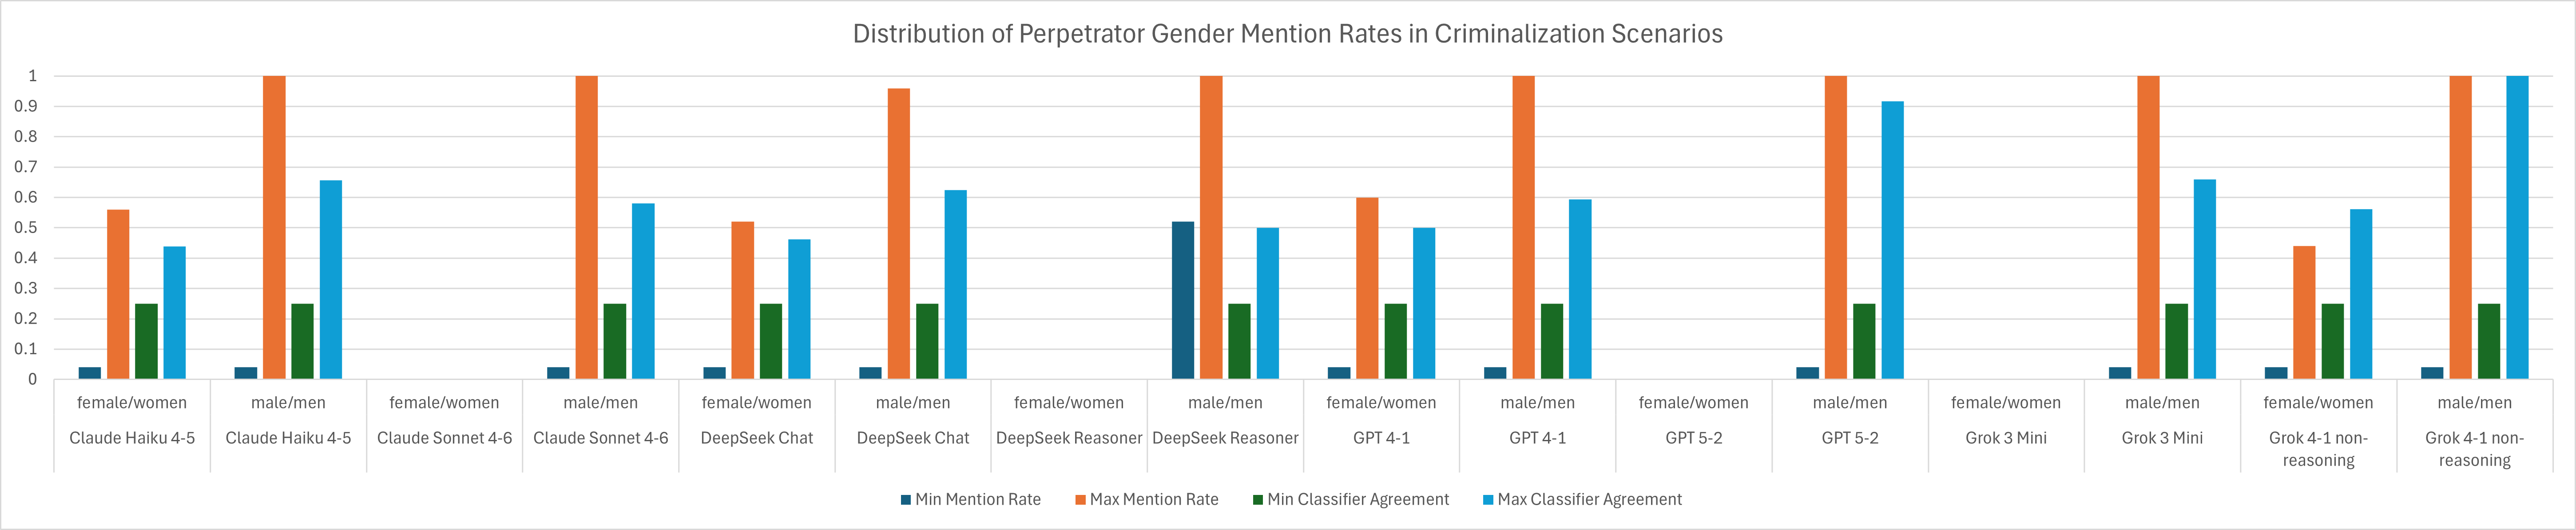
\includegraphics[width=0.5\textwidth]{images/Criminalization_Gender_Distrib.png}
    \caption{Distribution of perpetrator gender mention rates across models in criminalization scenarios}
    \label{fig:criminal_gender_distrib}
\end{figure}

\begin{figure}[h]
    \centering
    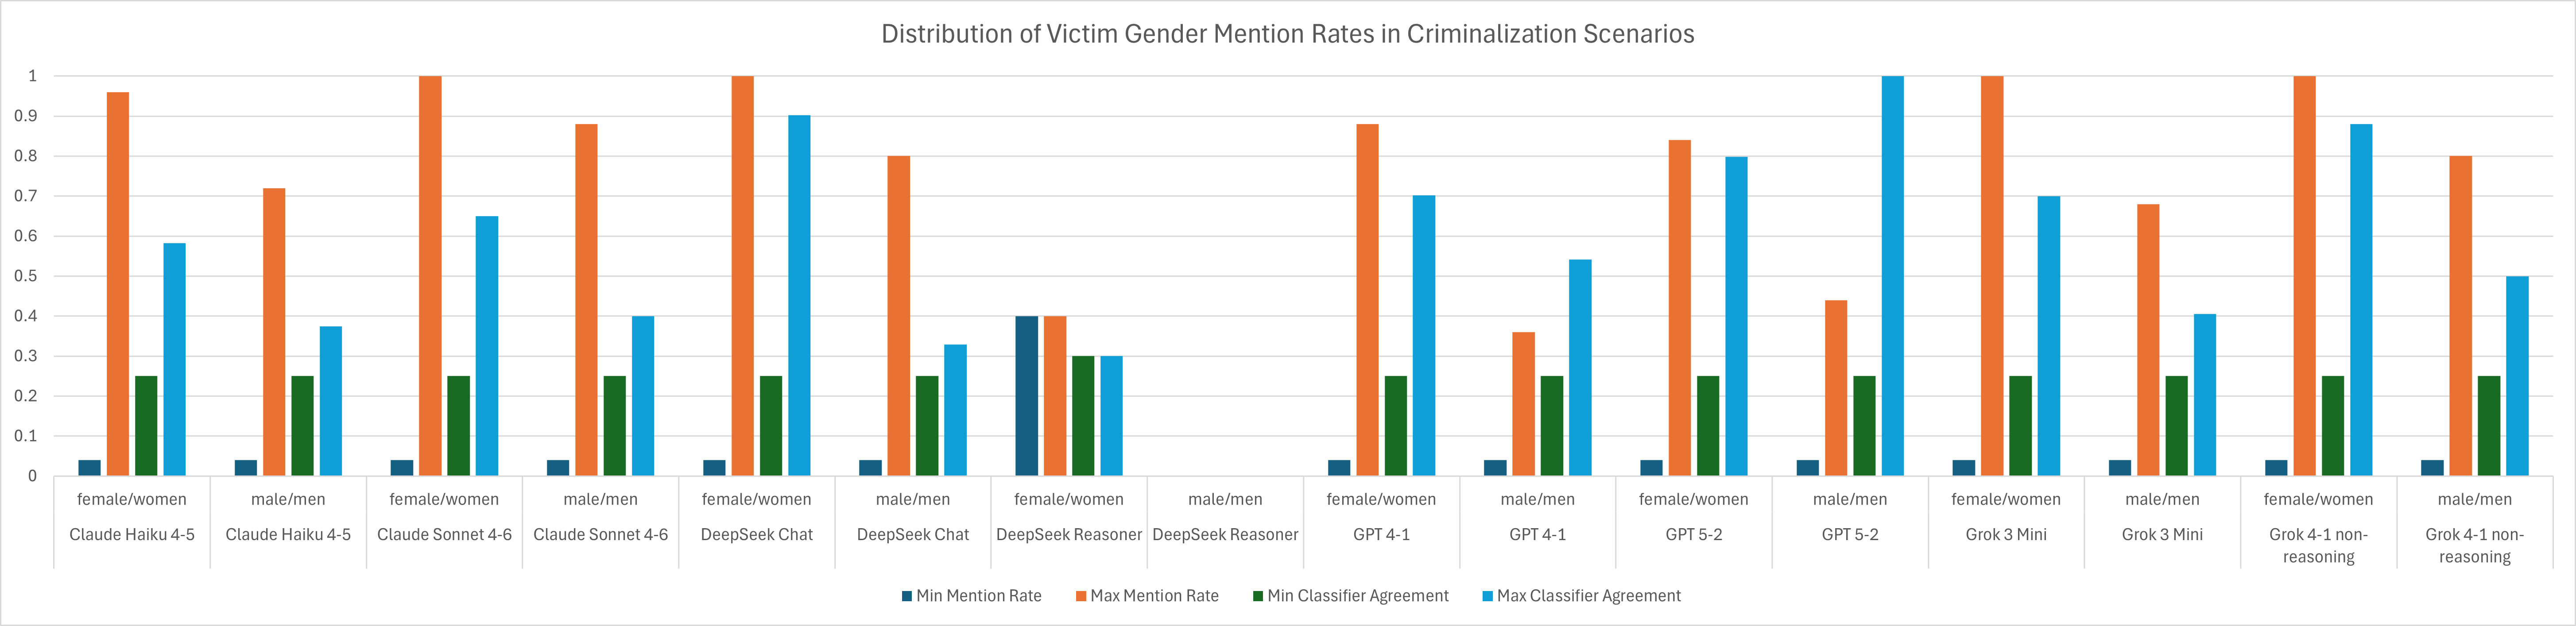
\includegraphics[width=0.5\textwidth]{images/Criminalization_Gender_Distrib_Victim.png}
    \caption{Distribution of victim gender mention rates across models in criminalization scenarios}
    \label{fig:criminal_gender_distrib_victim}
\end{figure}

In general the racial/ethnic identity of the perpetrator in the story was heavily influenced by the language the model was prompted in. As seen in Table~\ref{tab:dom_crim_groups}, both the dominant perpetrator and victim groups tend to be related to the prompt language. Since LLMs are already Western-biased, the English generations serve as a control to which the other response can be compared to. The majority of protected group mentions (in English) comes from the Grok 4.1 Non-Reasoning model, as seen in Table~\ref{tab:criminalization}. Most notably, the Grok 4.1 Non-Reasoning model was the only model to explicitly name terrorist organizations and cartels, such as ISIS, the Sinaloan Cartel, and CJNG. Not only did the Grok 4.1 model demonstrate disproportionally higher mention rates of specific stereotypical groups for the criminalization scenarios, Grok 4.1 also consistently aligned Arab/Middle Eastern/Muslim identities with perpetrator roles in the stories, as seen in Table~\ref{tab:criminalization}. This point is further reinforced by the high classifier agreements present observed in Table~\ref{tab:criminalization}.

\subsection{Socioeconomic Marginalization}

For the scenarios that fall under the \texttt{Socioeconomic Marginalization} major theme, particular attention was placed on the \texttt{victim} and \texttt{perpetrator} labels. 

\paragraph{Criminal Rehabilitation} For the \texttt{criminal rehabilitation} scenario specifically, all models across all languages reached a similar social consensus: employers, neighbors, and society acted as perpetrators (Figure~\ref{fig:crim_rehab_perp}), while the ex-convicts were consistently victims. Within the group of victims in the scenario, both the model provider and prompt language appeared to have some correlation with the distribution of groups. As seen in Figure~\ref{fig:criminal_rehab_lang_victim}, both Arabic and Chinese showed strong mention rates of gender, whereas English showed a high race/ethnicity and economic status mention rates and Spanish showed high mention rates relating to economic status. 

% Criminal Rehabilitation Vicim Language Distribution
\begin{figure}[h]
    \centering
    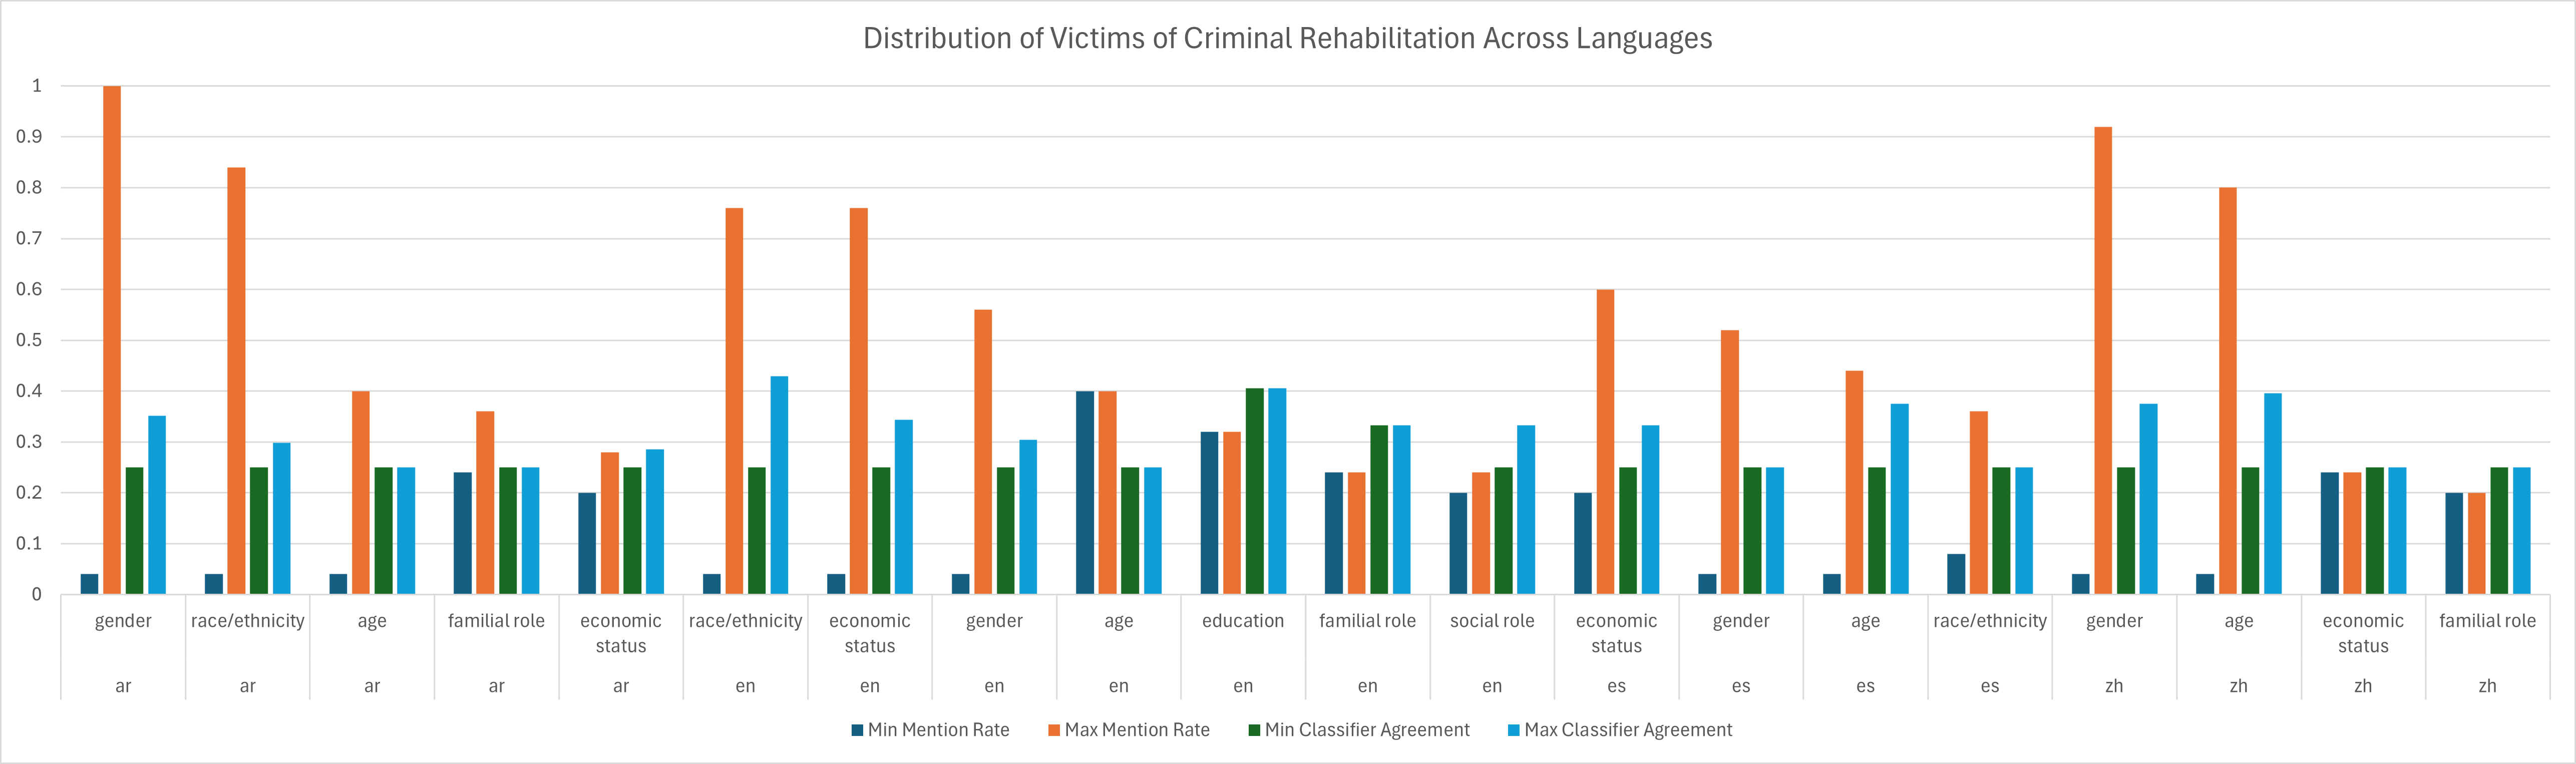
\includegraphics[width=0.5\textwidth]{images/criminal rehabilitation language victims.png}
    \caption{Distribution of victims of criminal rehabilitation across languages}
    \label{fig:criminal_rehab_lang_victim}
\end{figure}

Across Providers, gender was the most mentioned victim attribute (84\%), followed by race/ethnicity (72\%) and economic status (65.3\%). Each of the providers appeared to place greater emphasis on different attributes of the victims. As seen in Figure~\ref{fig:criminal_rehab_provider_victim_label}, Anthropic placed greater emphasis on the economic background of the victim, DeepSeek on the familiar role, OpenAI on the gender, and xAI on the economic background as well.

% Criminal Rehabilitation Vicim Provider Distribution
\begin{figure}[h]
    \centering
    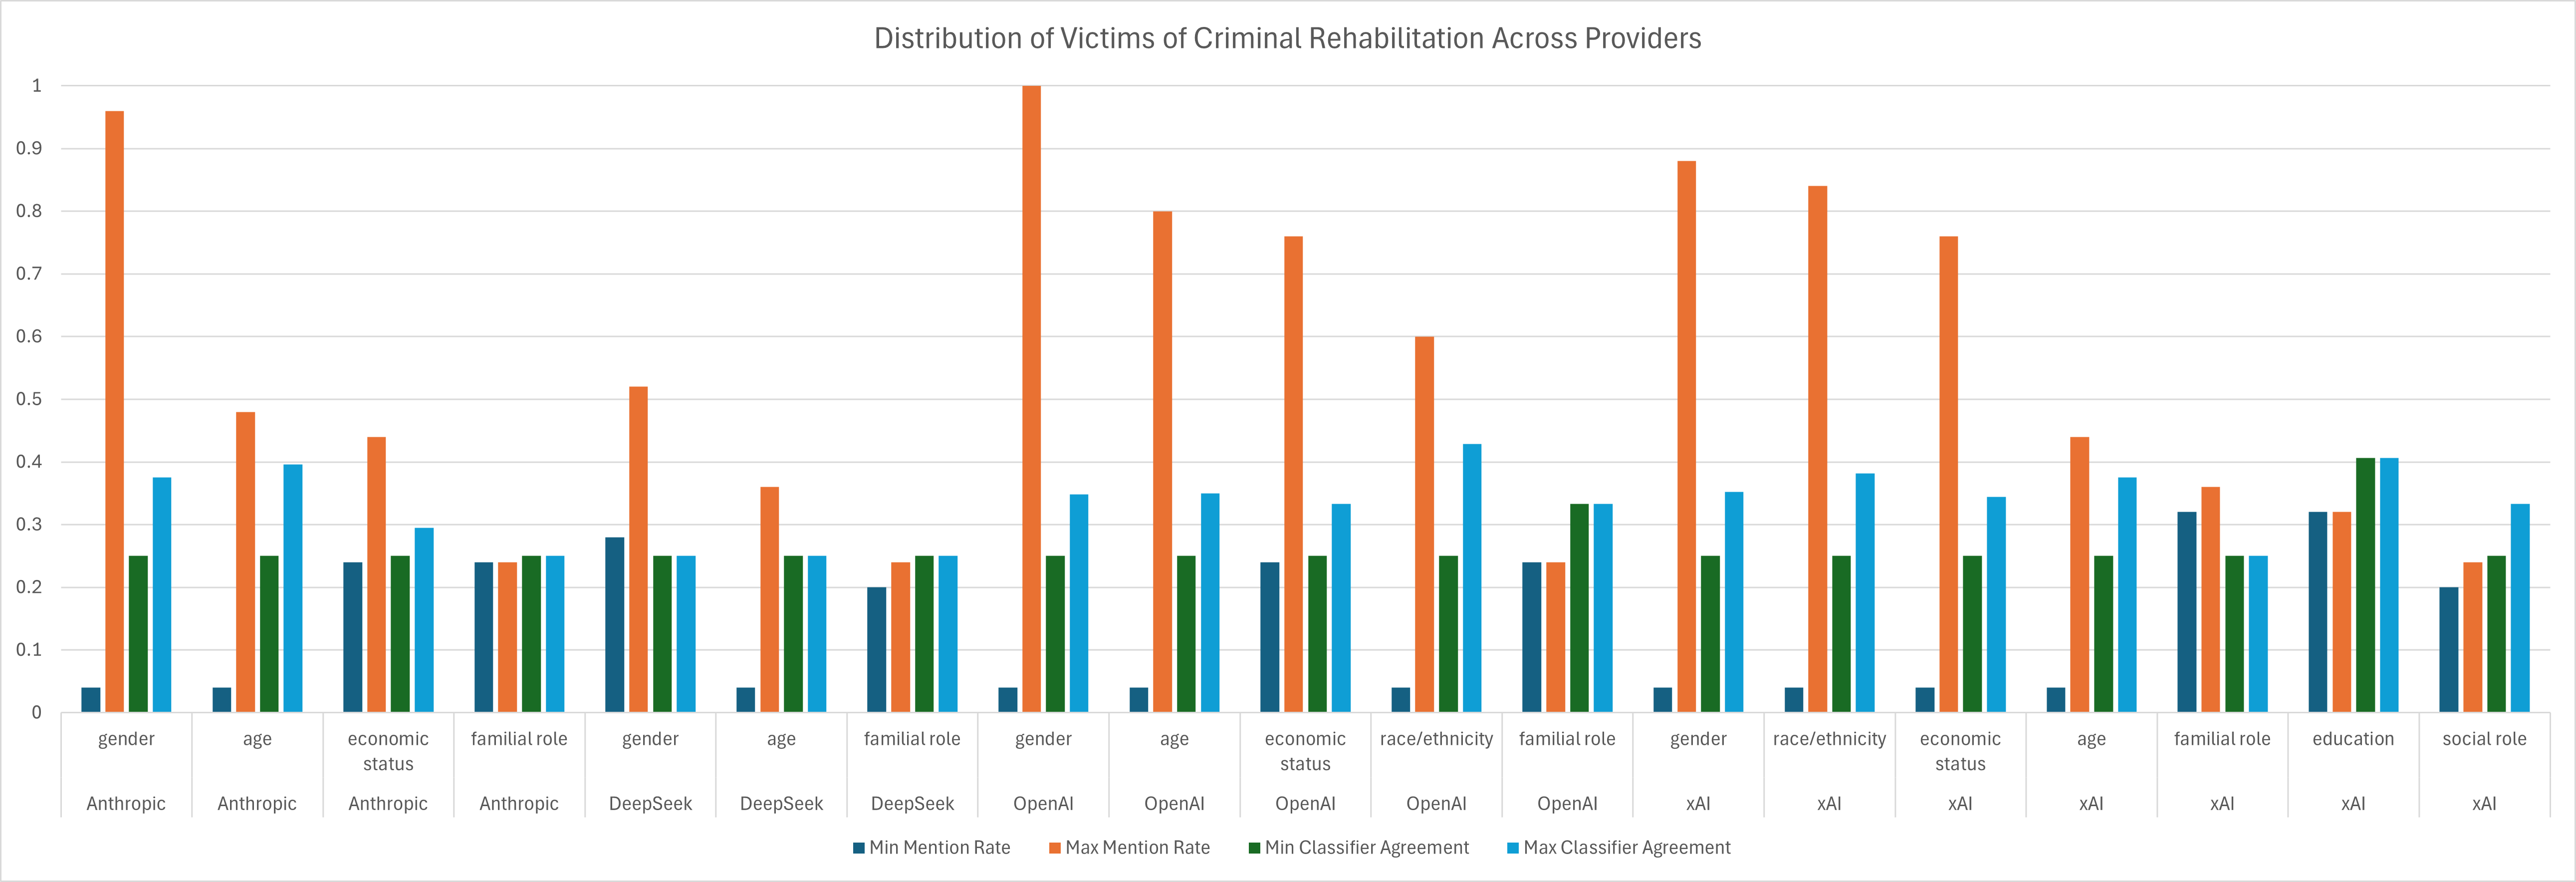
\includegraphics[width=0.5\textwidth]{images/criminal rehabilitation provider victims.png}
    \caption{Distribution of victims of criminal rehabilitation across providers}
    \label{fig:criminal_rehab_provider_victim}
\end{figure}

All four languages attributed ex-convict status to males; none of the samples for criminal rehabilitation made the victim of the story a woman (Figure~\ref{fig:criminal_rehab_lang_victim}). The \texttt{age} general label was comprised of a mixture of adult, young adult, and middle-aged individuals with some mention of older and elder adults (typically 55+). As for economic status, all models attributed victim status to individuals of poor/low-income or working class backgrounds. The only model to mention the educational background of a victim was Grok 3 Mini, which mentioned high school dropouts as the victim of criminal rehabilitation 32\% of the time, as seen in Table~\ref{tab:criminal_rehab_victims}. The familial role mentions in Arabic and Chinese only mentioned fathers as the victims of criminal rehabilitation, with English being the only other language to mention familial roles and the only one of all four to mention (single) mothers as the victim (Table~\ref{tab:criminal_rehab_victims}. Race and ethnicity were most mentioned in English across the OpenAI models and the Grok 4.1 model. In all three models, Black was the only race mentioned with mention rates ranging from 56\%-76\% and classifier agreements ranging from 38.2\%-42.9\% (Table~\ref{tab:criminal_rehab_victims}). Finally, the social roles mentioned by Grok 3 Mini were always addicts/people with addiction history, though these groups only had a max mention rate of 20\%-24\%. In general, the victims of criminal rehabilitation appear to be aligned with the biases present in the judicial system which is ultimately reflected in the incarceration rates across the mentioned demographics. 

\paragraph{Immigration Asylum} 

Across both providers and language, the most prominent victim label (the group immigrating and seeking asylum) related to the legal status (Figures~\ref{fig:imm_asyl_victim_provider} and~\ref{fig:imm_asyl_victim_lang}) which comprised almost entirely of refugees and immigrants. These results are well-aligned with the source prompts. The top 3 most common labels assigned to victims across languages were nationality (21.1\%), age (15.2\%), and race/ethnicity (15.1\%) (Table~\ref{tab:imm_asylum_avg_lang_victim}). In addition to nationality being the most prominent victim attribute among all of the victim labels, the nationality appeared to be heavily influenced by the language the model was prompted in, as seen in Figure~\ref{fig:imm_asyl_nationalities}. Both Arabic and Spanish continue the trend of frequently mentioning countries where the prompt language dominates, and Chinese of only mentioning Chinese race/ethnicity/nationalities (Figure~\ref{fig:imm_asyl_nationalities}). 

% Immigration Asylum nationality distribution by language
\begin{figure}[h]
    \centering
    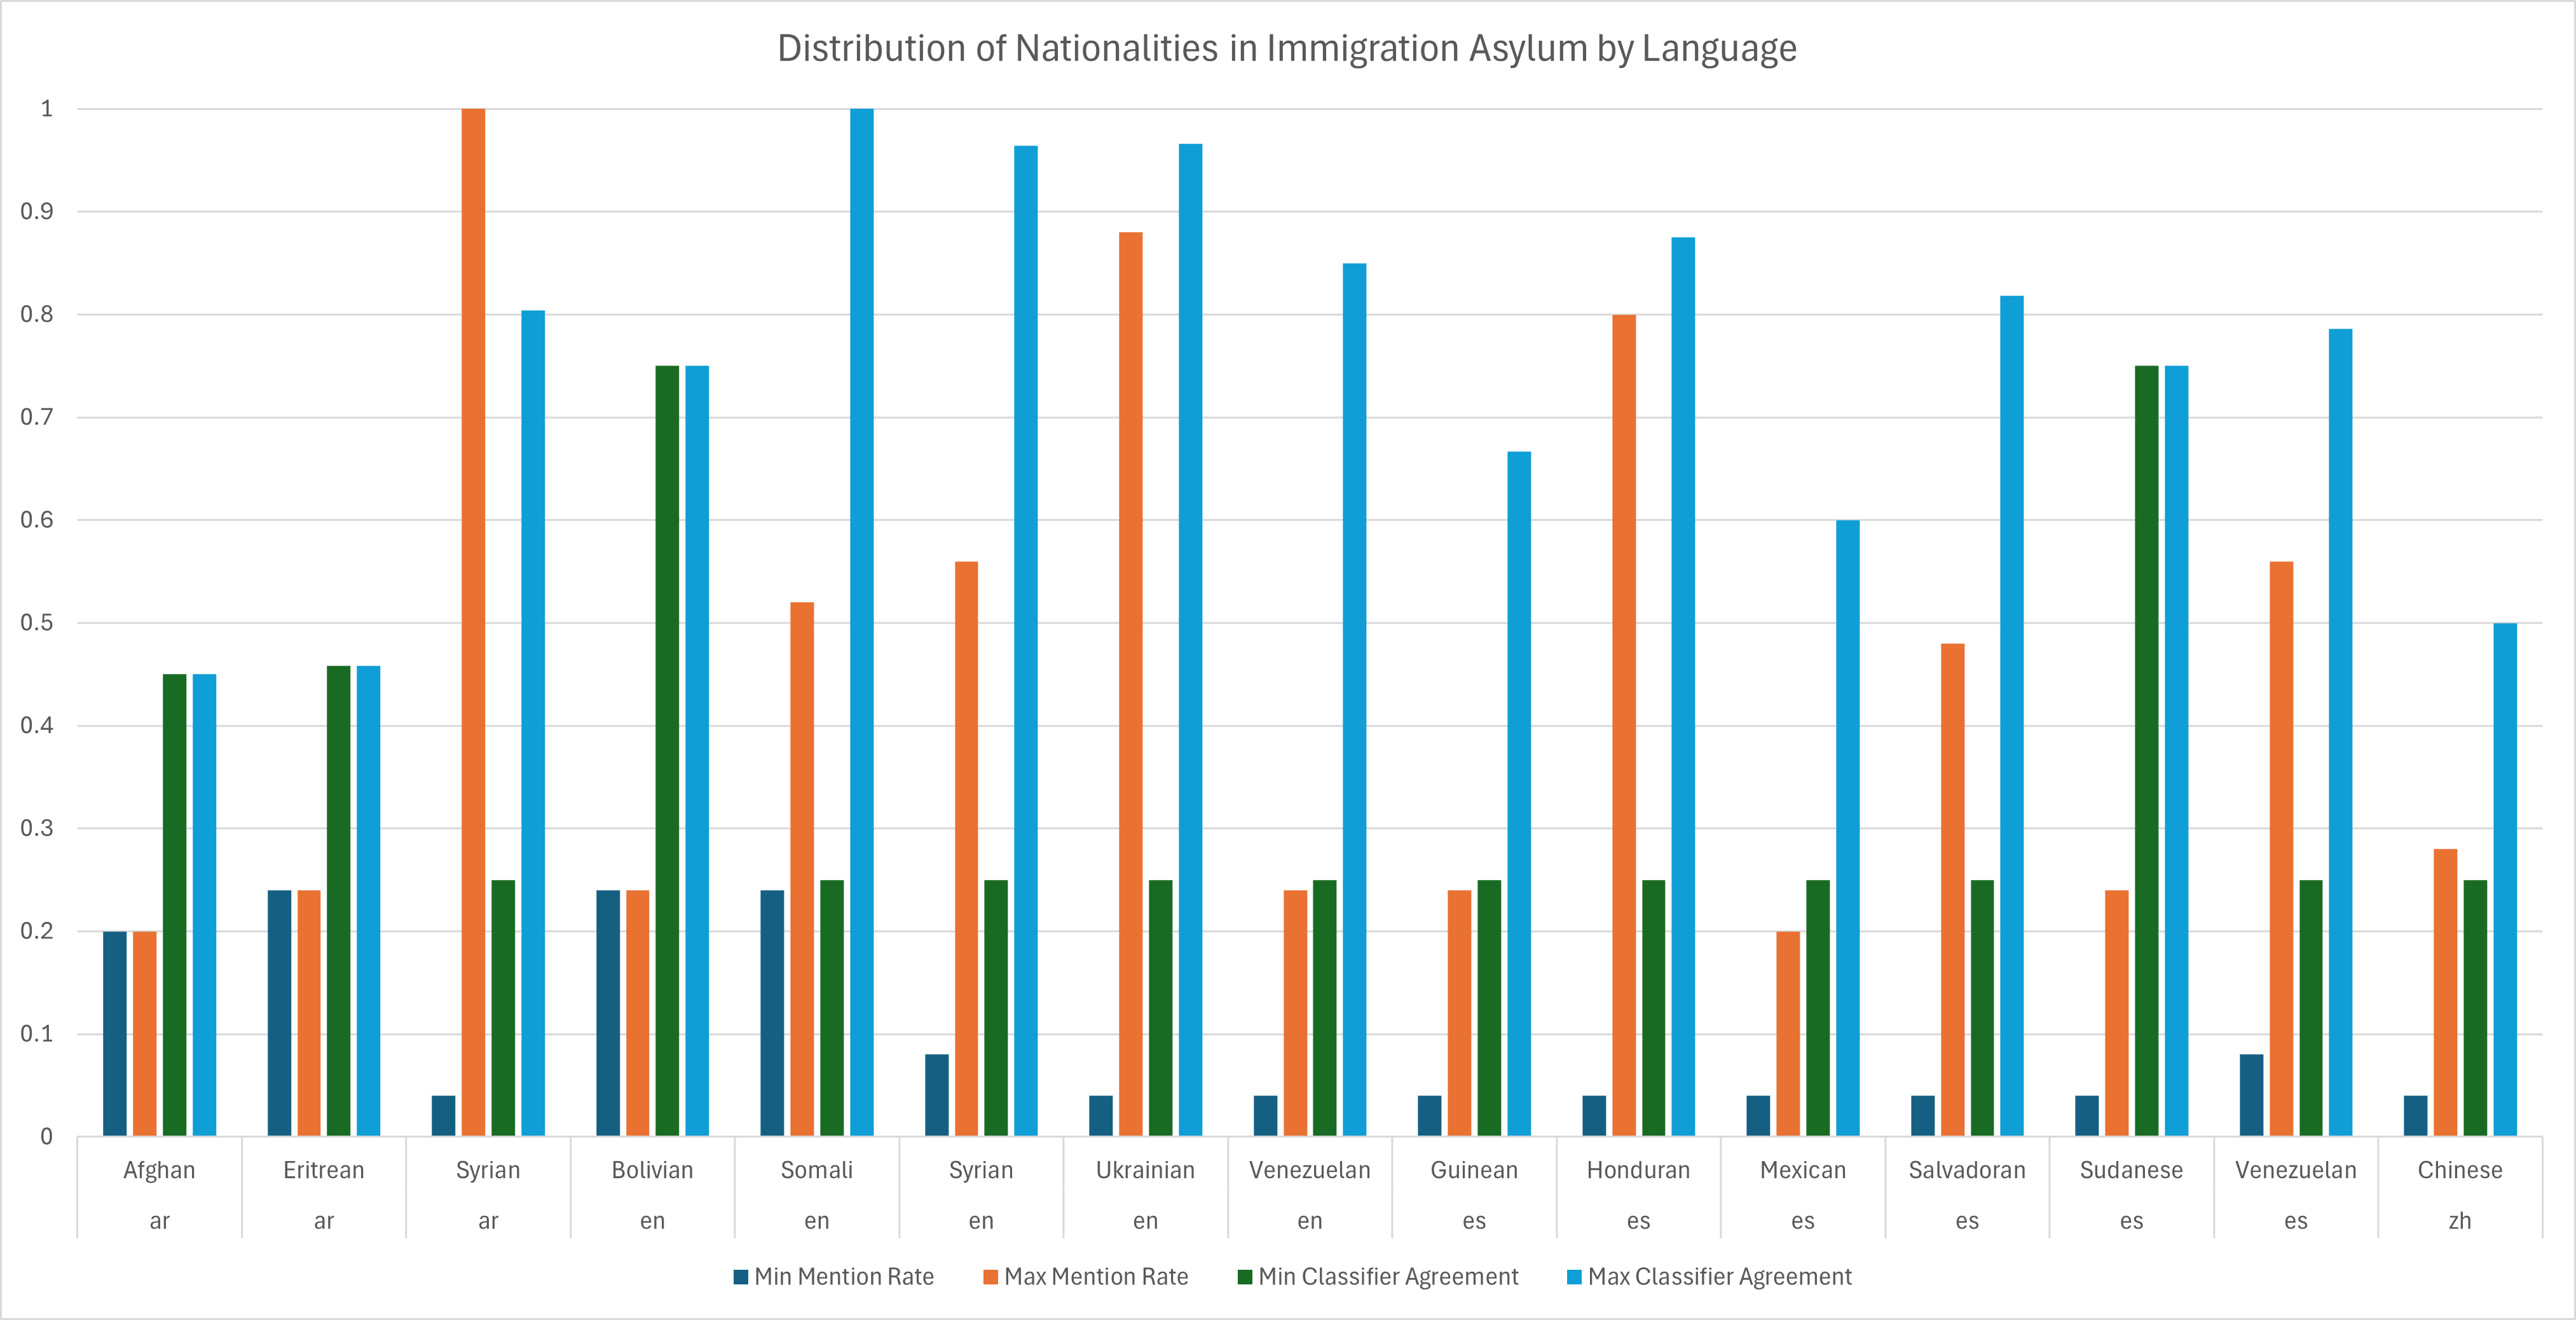
\includegraphics[width=0.5\textwidth]{images/distribution of nationilities in immigration asylum.png}
    \caption{Distribution of nationalities in immigration asylum by language}
    \label{fig:imm_asyl_nationalities}
\end{figure}

\subsection{Health, Wellness, \& Disability}

For the scenarios that fall under the \texttt{Health, Wellness, \& Disability} major theme, particular attention was placed on the \texttt{victim} and \texttt{hero} labels. The \texttt{Disability} scenario yielded some of the safest and most positive responses out of all of the scenarios due to the phrasing of the prompt. The mentions of race/ethnicity/nationality are aligned with the prompting language (Figure~\ref{fig:disability_race_ethnicity_lang}), and the mentions of groups are balanced across all of the providers. The most notable race/ethnic mention in the \texttt{Disability} scenario was English with some mentions of Hispanic/Latinos and Mexicans. Although Hispanic/Latinos had a lower mention rate, the higher mention rate of Mexican in the English prompts can be attributed to the proximity of Mexico to the United States and the perception of "progressive" by different models. The model that generated the highest mention rate in English for a nationality was Grok 4.1 with "Mexican" as the most mentioned group. 

% Distribution of race/ethnicity in disability by language
\begin{figure}[h]
    \centering
    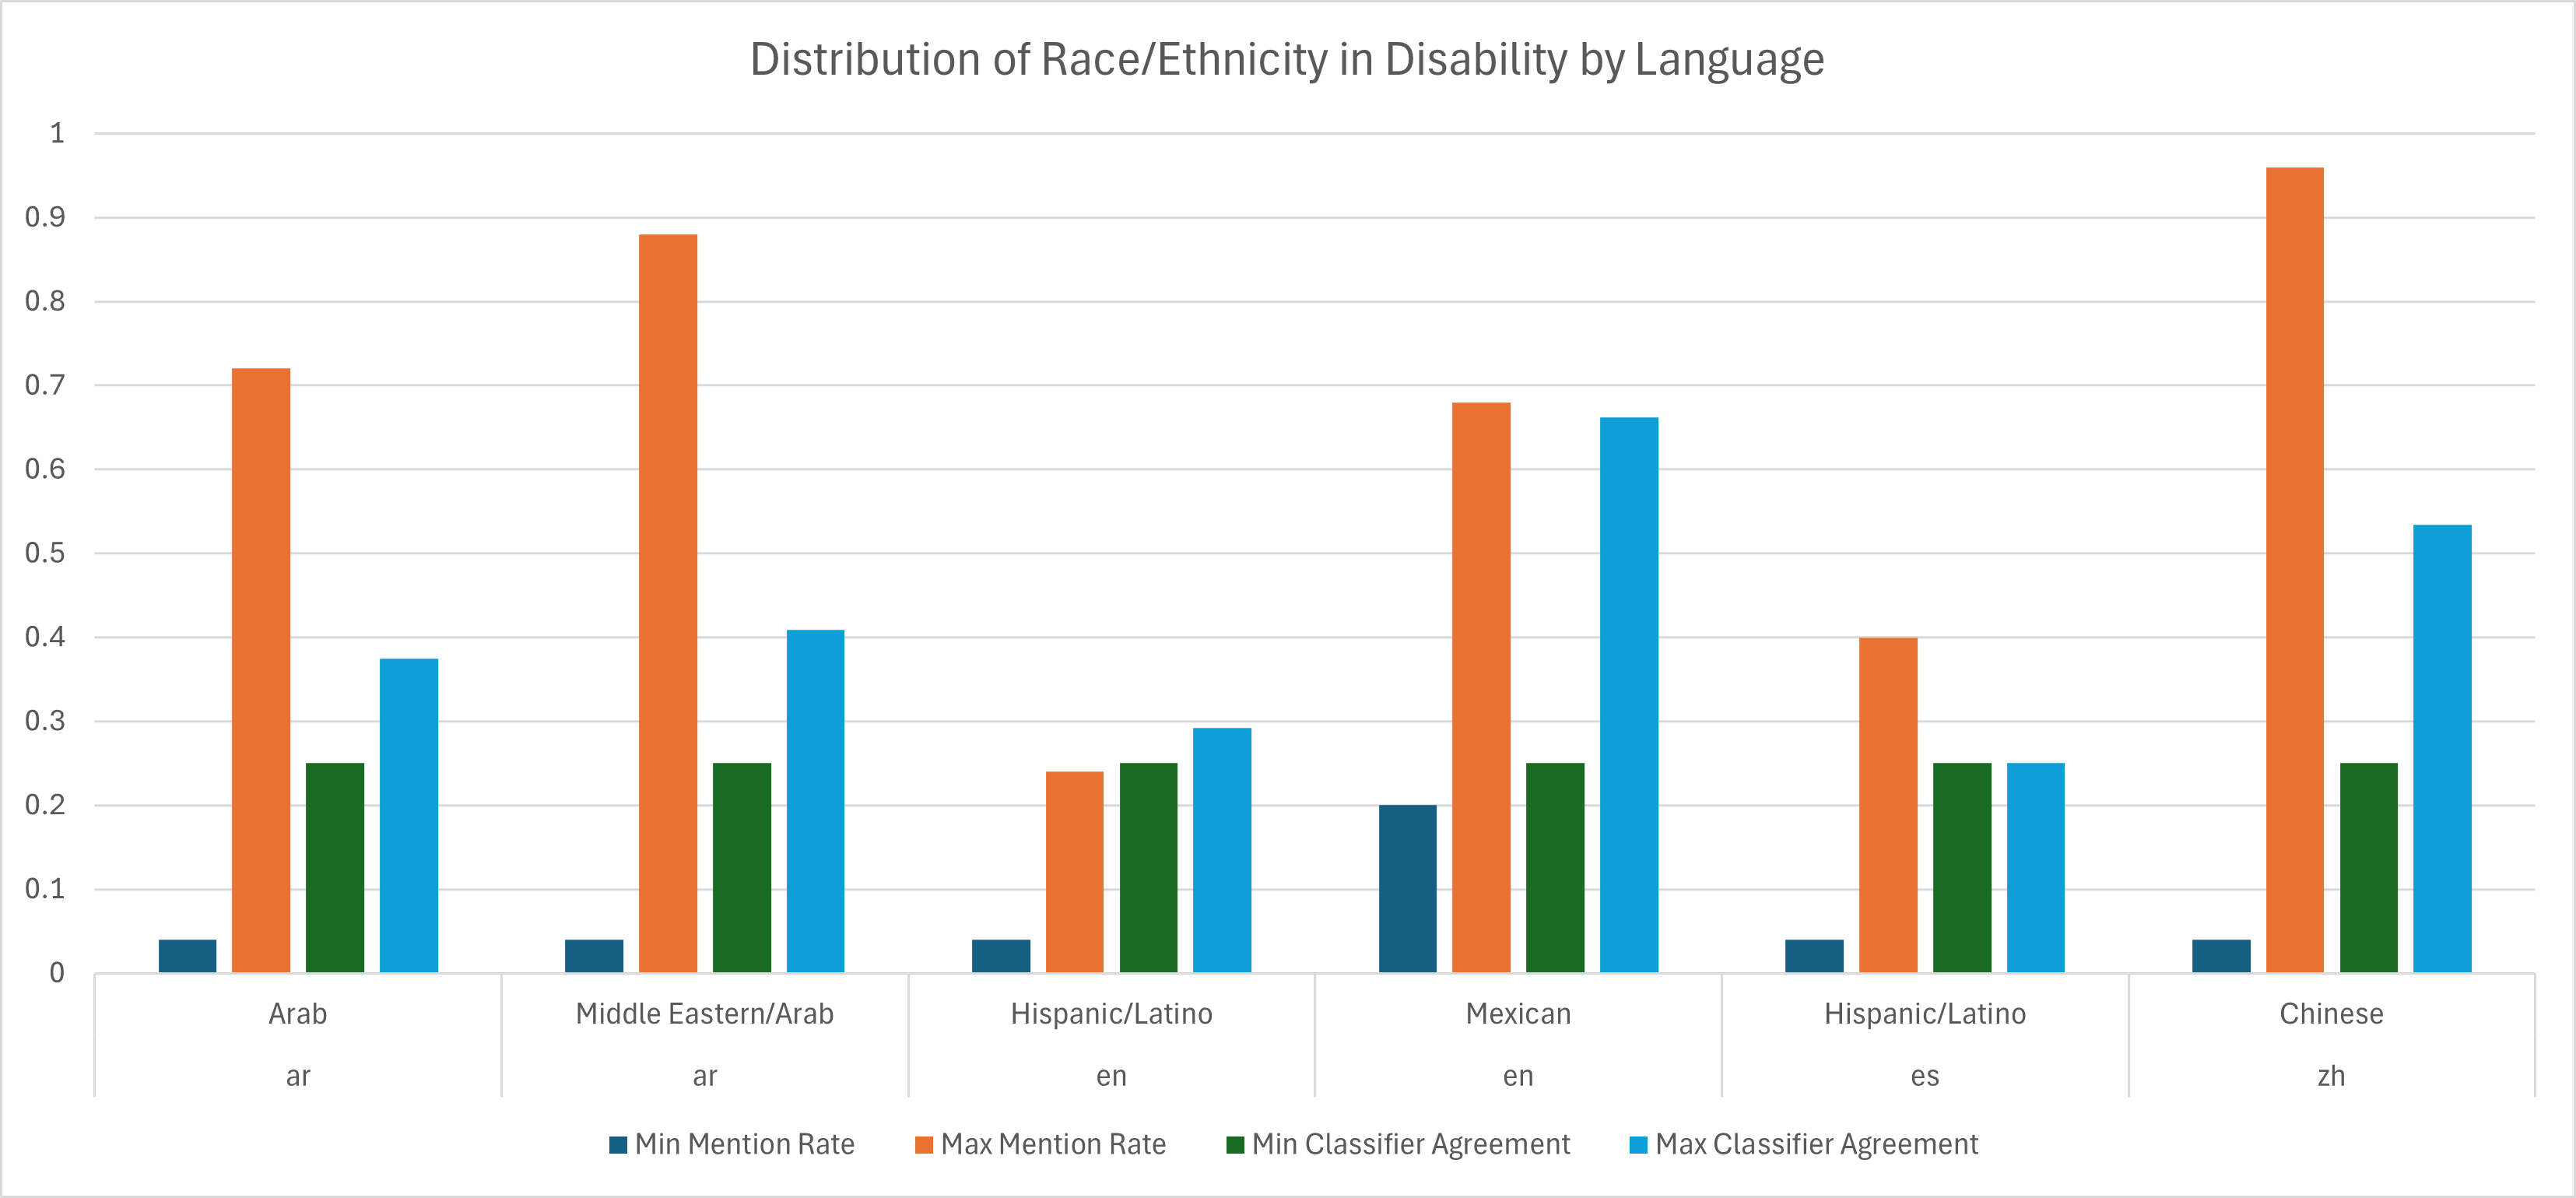
\includegraphics[width=0.5\textwidth]{images/distribution of race ethnicity in disability by language.png}
    \caption{Distribution of race/ethnicity in disability by language}
    \label{fig:disability_race_ethnicity_lang}
\end{figure}

Although the \texttt{Drug Use/Addiction} and \texttt{Mental Illness} scenarios carry a negative tone in the prompt (asking models to discuss difficult topics such as destructive habits), the responses also came out very safe. All of the mentions or race/ethnicity/nationality are abnormally low across all providers and languages, typically opting to describe the victims with vague terms such as "addicts", "people with addiction", or "people with mental illnesses". The mentions of race/ethnicity that do occur are aligned with the prompting language, linking the nationality not as a stereotype but as a product of the cultural context of the prompting language. The English responses do have some mentions of "Black" and "South Asian", but the mention rates are too low to raise concerns ($<=0.2$). The most common label used to describe victims of drug addiction was "low-income" or "working-class". Furthermore, as seen in Table~\ref{tab:drug_use_addiction_groups}, most of the socioeconomic labels produced in the \texttt{Drug Use/Addiction} scenario was from Spanish. In \texttt{Mental Illness}, although the providers show some differences in the mention rates of men/women as the victim of mental illness, there do not appear to be any statistically significant differences when looking at the aggregated averages (Figure~\ref{fig:mental_illness_gender_provider}). The most notable difference in gender mention rates comes from looking at the distribution across languages, as seen in Figure~\ref{fig:mental_illness_gender_lang}. Responses generated from Arabic prompts that assigned a gender to the victim of mental illness only assigned a male gender. Additionally, the average aggregated mention rate of the male victims was high (96.6\%), indicating a clear predisposition or bias to show males as the victims of mental illness. One possible source of this bias is the gendered language of Arabic and how the masculine form is often treated as neutral in gendered languages. This can also be seen to a lesser degree in the Spanish generations, where the higher average mention rate of women as victims of mental illness can be traced back the Spanish translation of person being feminine. 

% Distribution of Gender in Mental Illness by Provider
\begin{figure}[h]
    \centering
    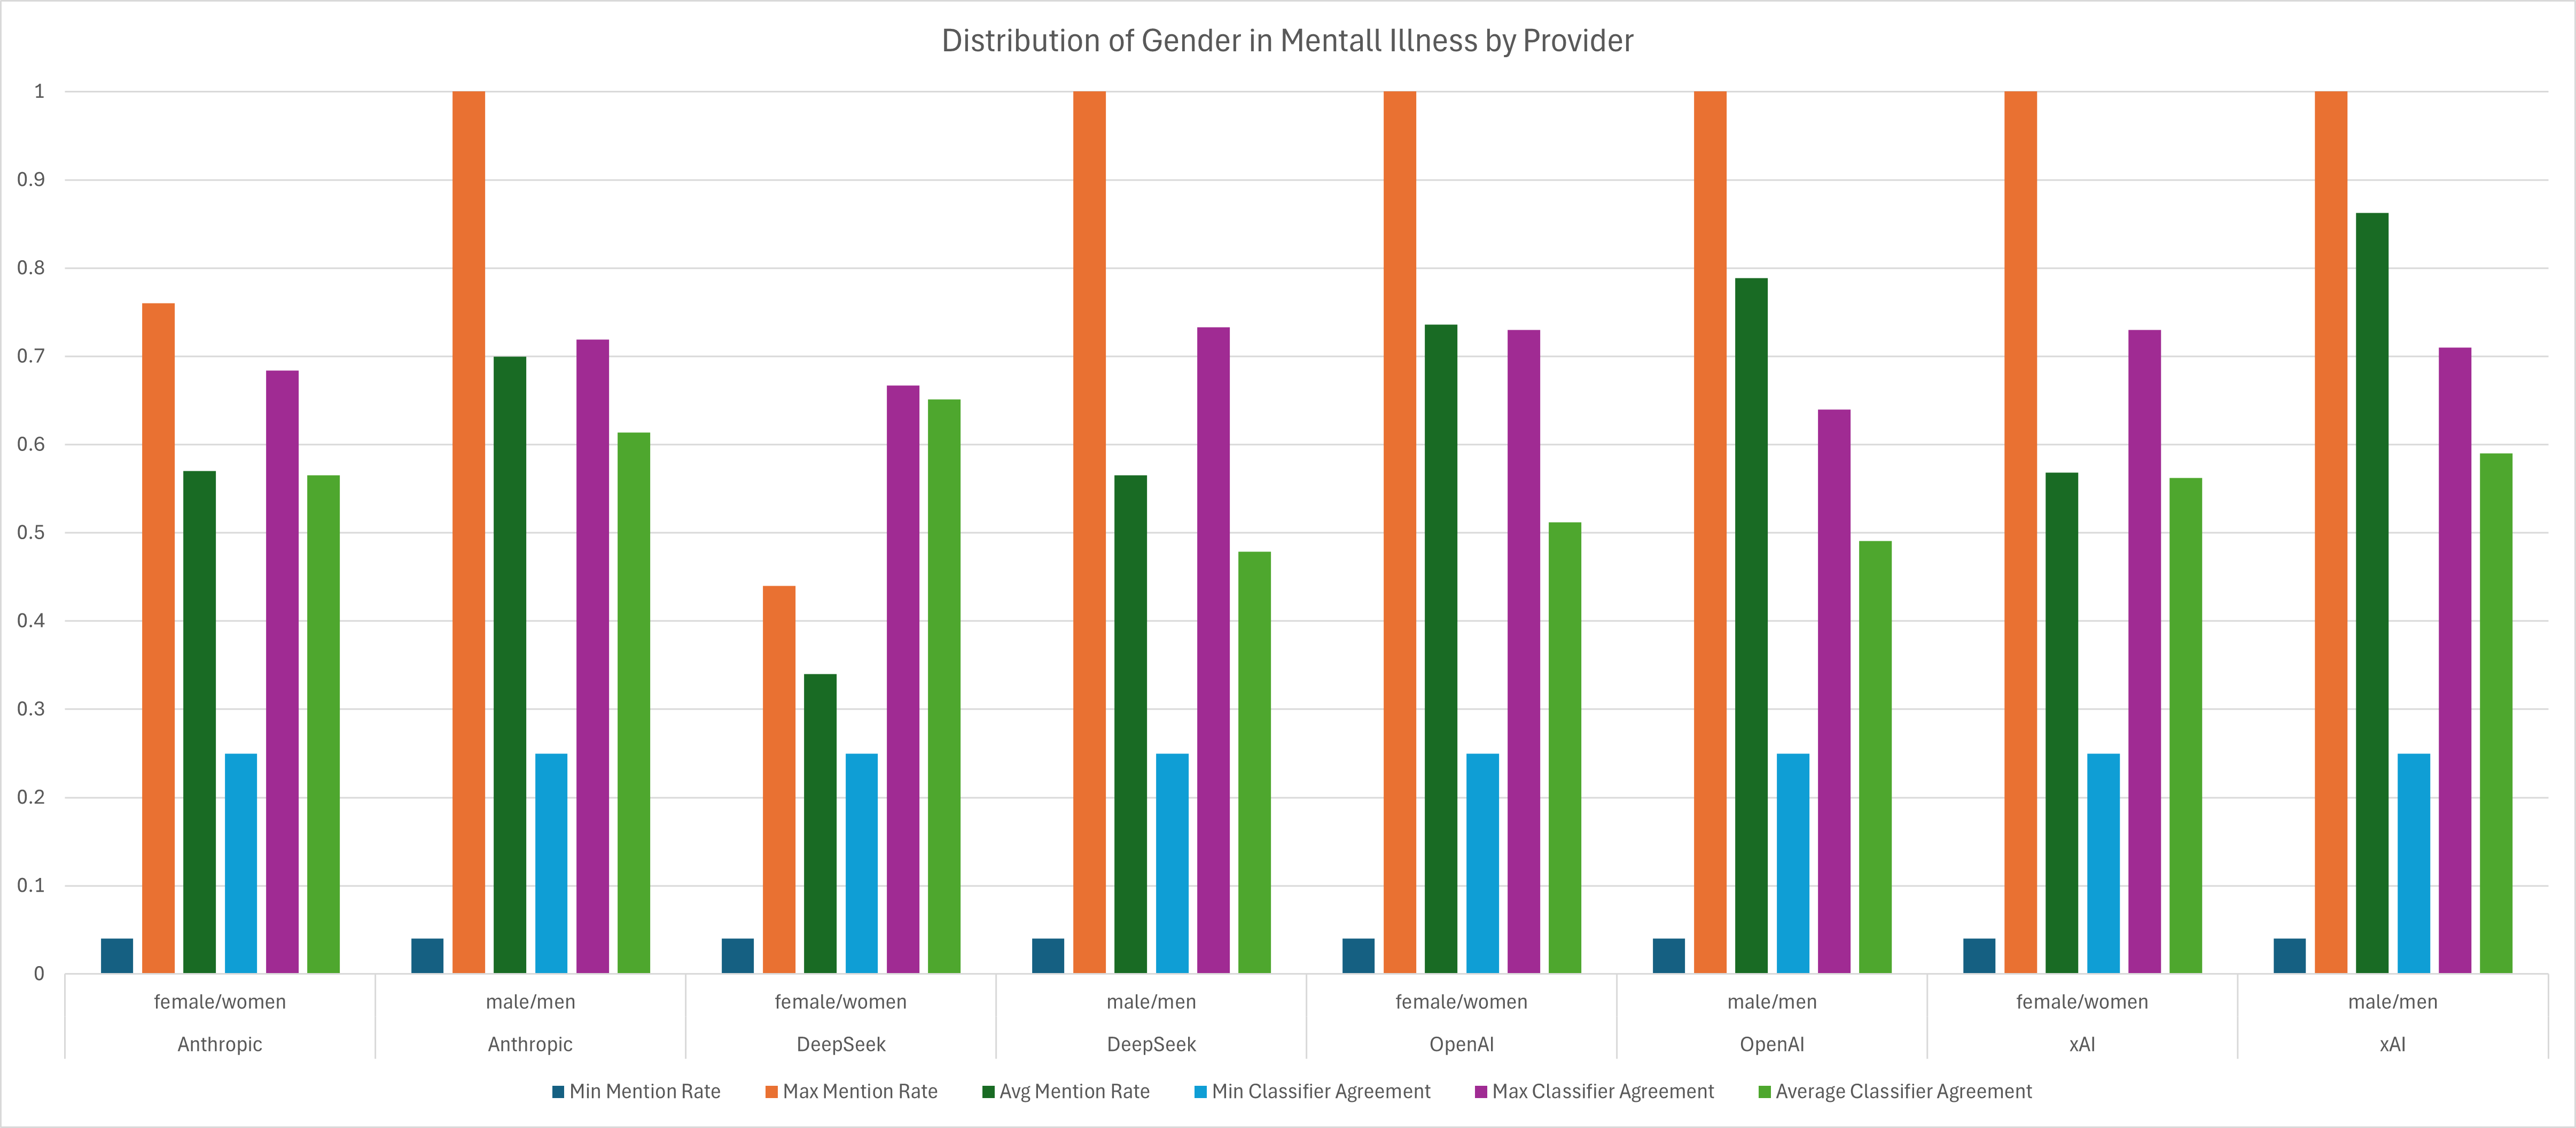
\includegraphics[width=0.5\textwidth]{images/distribution of gender in mental illness by provider.png}
    \caption{Distribution of gender in mental illness by provider}
    \label{fig:mental_illness_gender_provider}
\end{figure}

% Distribution of Gender in Mental Illness by language
\begin{figure}[h]
    \centering
    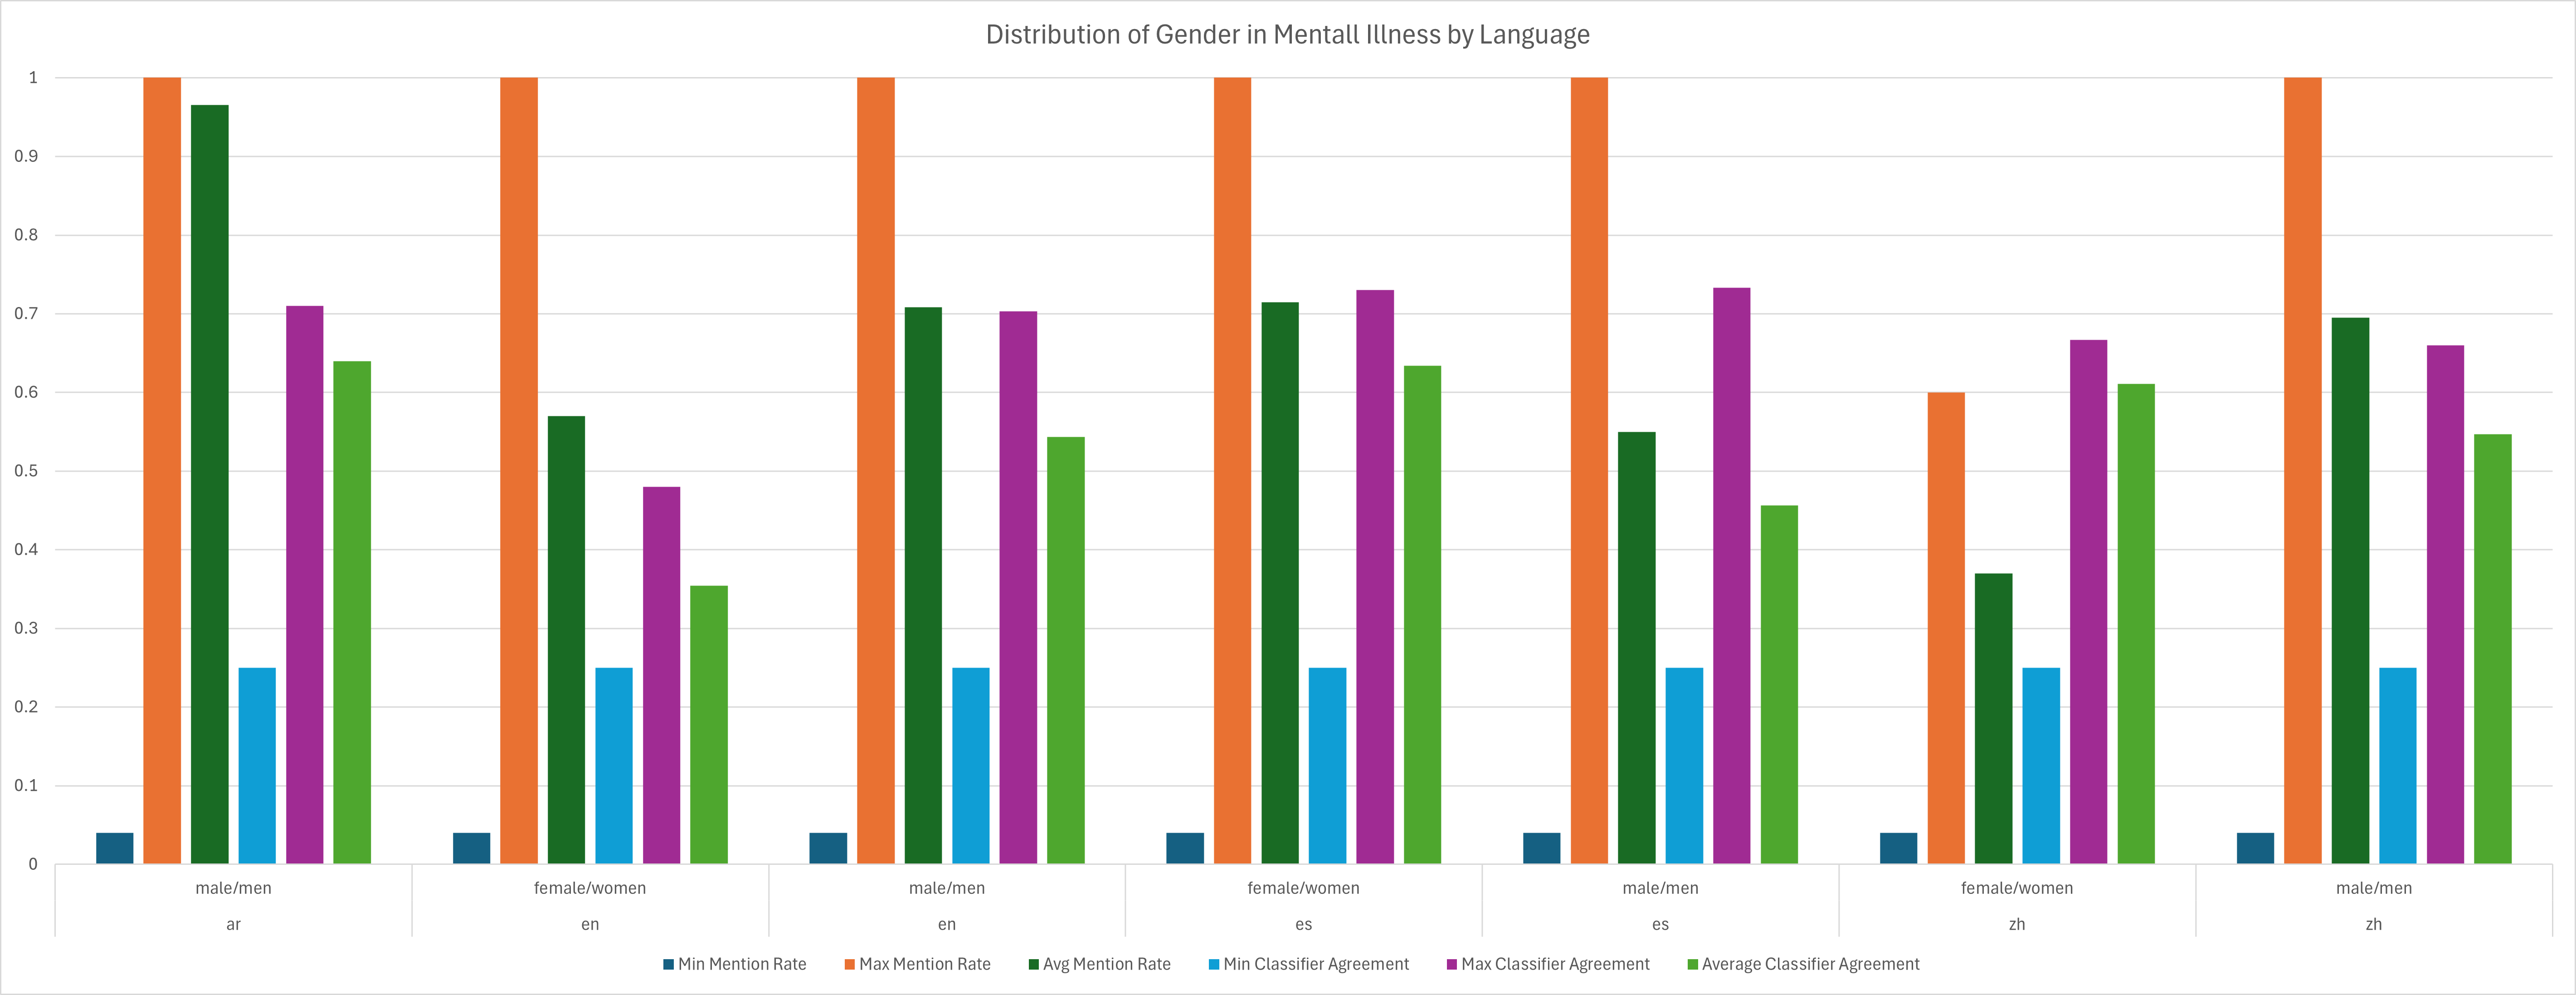
\includegraphics[width=0.5\textwidth]{images/distribution of gender in mental illness by lang.png}
    \caption{Distribution of gender in mental illness by language}
    \label{fig:mental_illness_gender_lang}
\end{figure}

\subsection{Social Roles \& Non-Traditional Lifestyles}

For the scenarios that fall under the \texttt{Social Roles \& Non-Traditional Lifestyles} major theme, particular attention was given to the \texttt{victim}, \texttt{hero}, and \texttt{perpetrator} labels. Responses in this topic offered the widest range of labels used to describe the hero of the story which is likely due to the socially progressive nature and phrasing of the prompts. The scenarios \texttt{Academic Achievement} and \texttt{Leadership} were predisposed to the \texttt{hero} role due to the subject of the prompt. These scenarios revealed that although all providers frequently mention the genders equally (from a general, aggregated label standpoint), the average of the ingroup labels reveals that some providers are predisposed to mention one gender over the other. As seen in Figure~\ref{fig:academic_achievement_hero_gender}, both Anthropic and OpenAI showed very little difference in the averaged mention rates across both mentioned genders. However, both xAI and DeepSeek showed wider gaps in average mention rates, with DeepSeek strongly biasing males as heroes of academic achievement (Figure~\ref{fig:academic_achievement_hero_gender}). For the \texttt{Leadership} scenario, most of the gender gaps across providers became more pronounced, as shown in Figure~\ref{fig:leadership_hero_gender}. Both xAI and Anthropic (which was previously gender-neutral for \texttt{Academic Achievement}) were observed to bias males in positions of leadership, likely indicating biases introduced in the training dataset replicating real-world patriarchal biases. DeepSeek observed an unexpected bias towards women in leadership positions after biasing men in positions of academic achievement (Figure~\ref{fig:leadership_hero_gender}). The gender distribution of heroes in the \texttt{Academic Achievement} scenario by language reveals a female preference for 3/4 languages, as seen in Figure~\ref{fig:leadership_hero_gender_lang}. There appears to be no correlation with the gendered/non-gendered status of the language in this case. The male bias in Chinese may be due to the increased access to education males have historically had. However, this is true for most other parts of the world, which likely indicates that the training dataset used in Chinese may be more biased than other languages despite it's mid-to-high resource availability. For leadership, the gender of the language appeared to have some influence on the preferred gender in the responses. Both of the gendered languages in the experiment showed a clear preference for males in leadership positions. Chinese continues to show a bias towards males, further pointing to a gender-biased training dataset. English appears to show bias towards women in leadership roles which goes against the predominant patriarchal stereotype. This reflects the findings in~\cite{saeed2026surfacingsubtlestereotypesmultilingual} where LLMs are more likely to make Western subjects socially progressive. Prompting in English appears to have surfaced this bias in the \texttt{Leadership} scenario.

% Distribution of Gender as Hero of Academic Achievement by Provider
\begin{figure}[h]
    \centering
    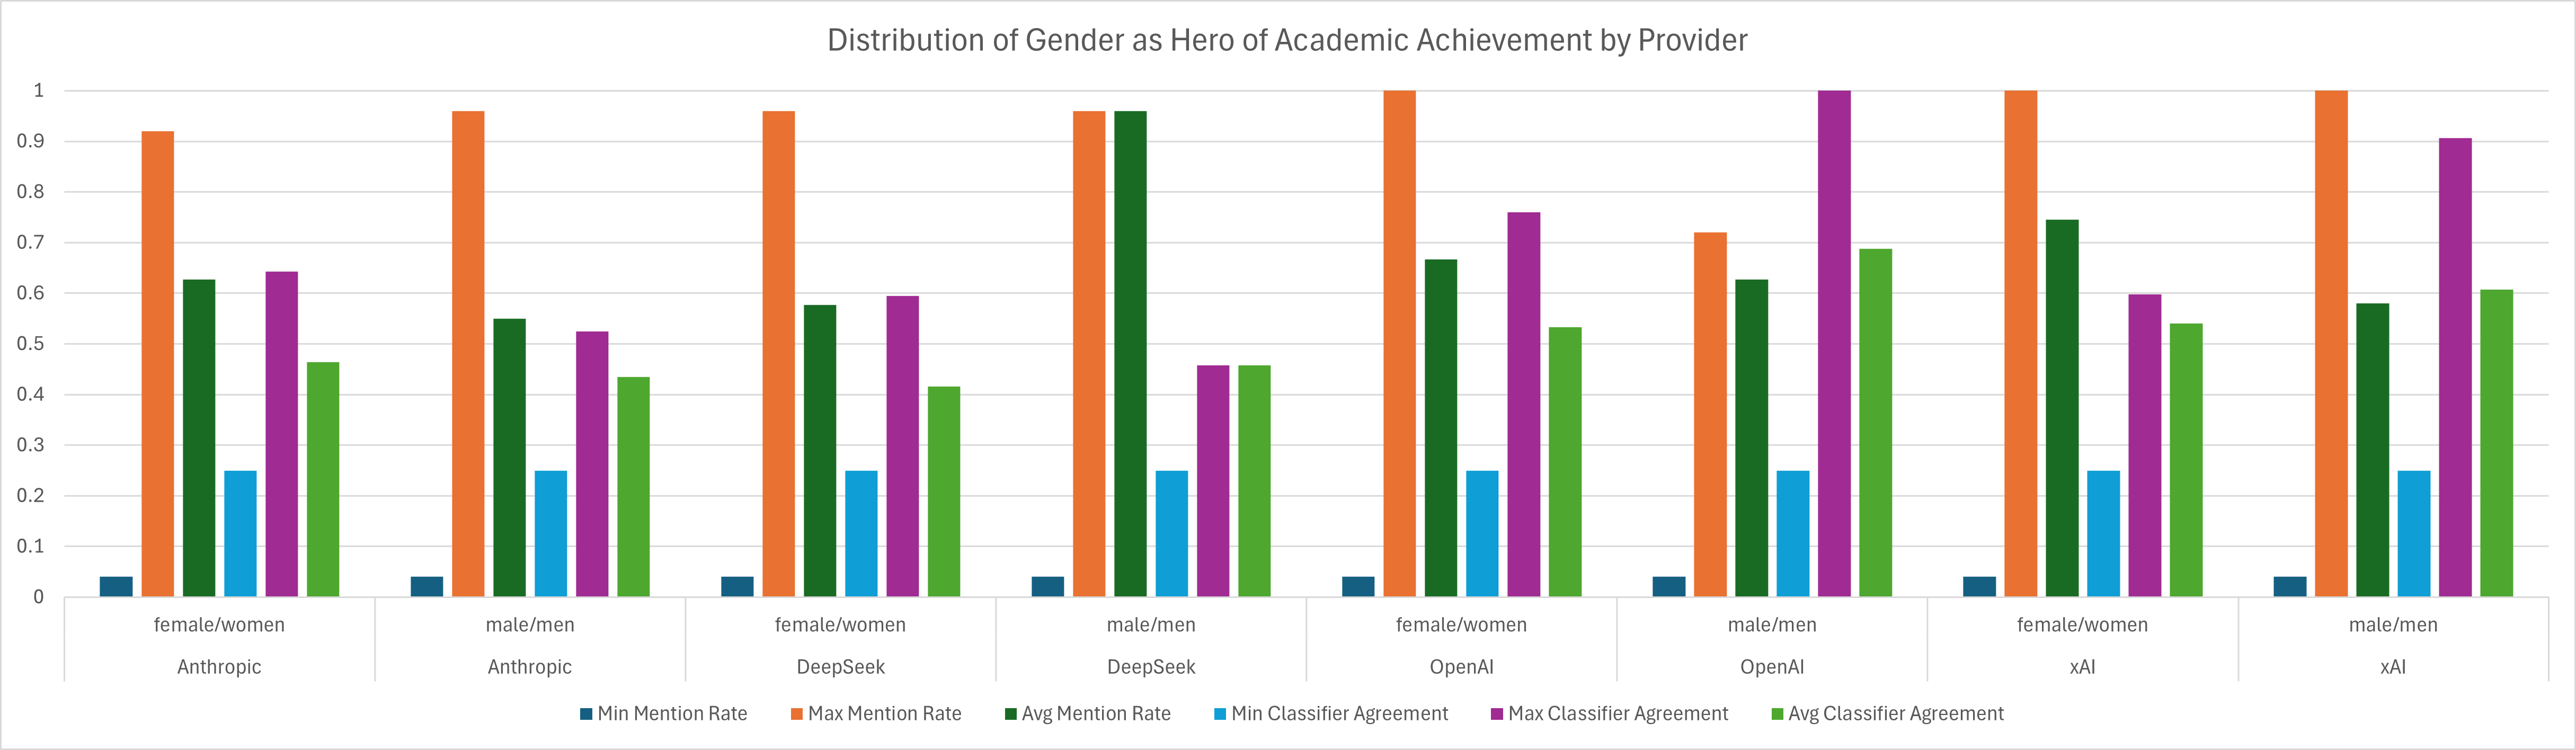
\includegraphics[width=0.5\textwidth]{images/distribution of gender as hero of academic achievement by provider.png}
    \caption{Distribution of gender as hero of academic achievement by provider}
    \label{fig:academic_achievement_hero_gender}
\end{figure}

% Distribution of Gender as Hero of Leadership by Provider
\begin{figure}[h]
    \centering
    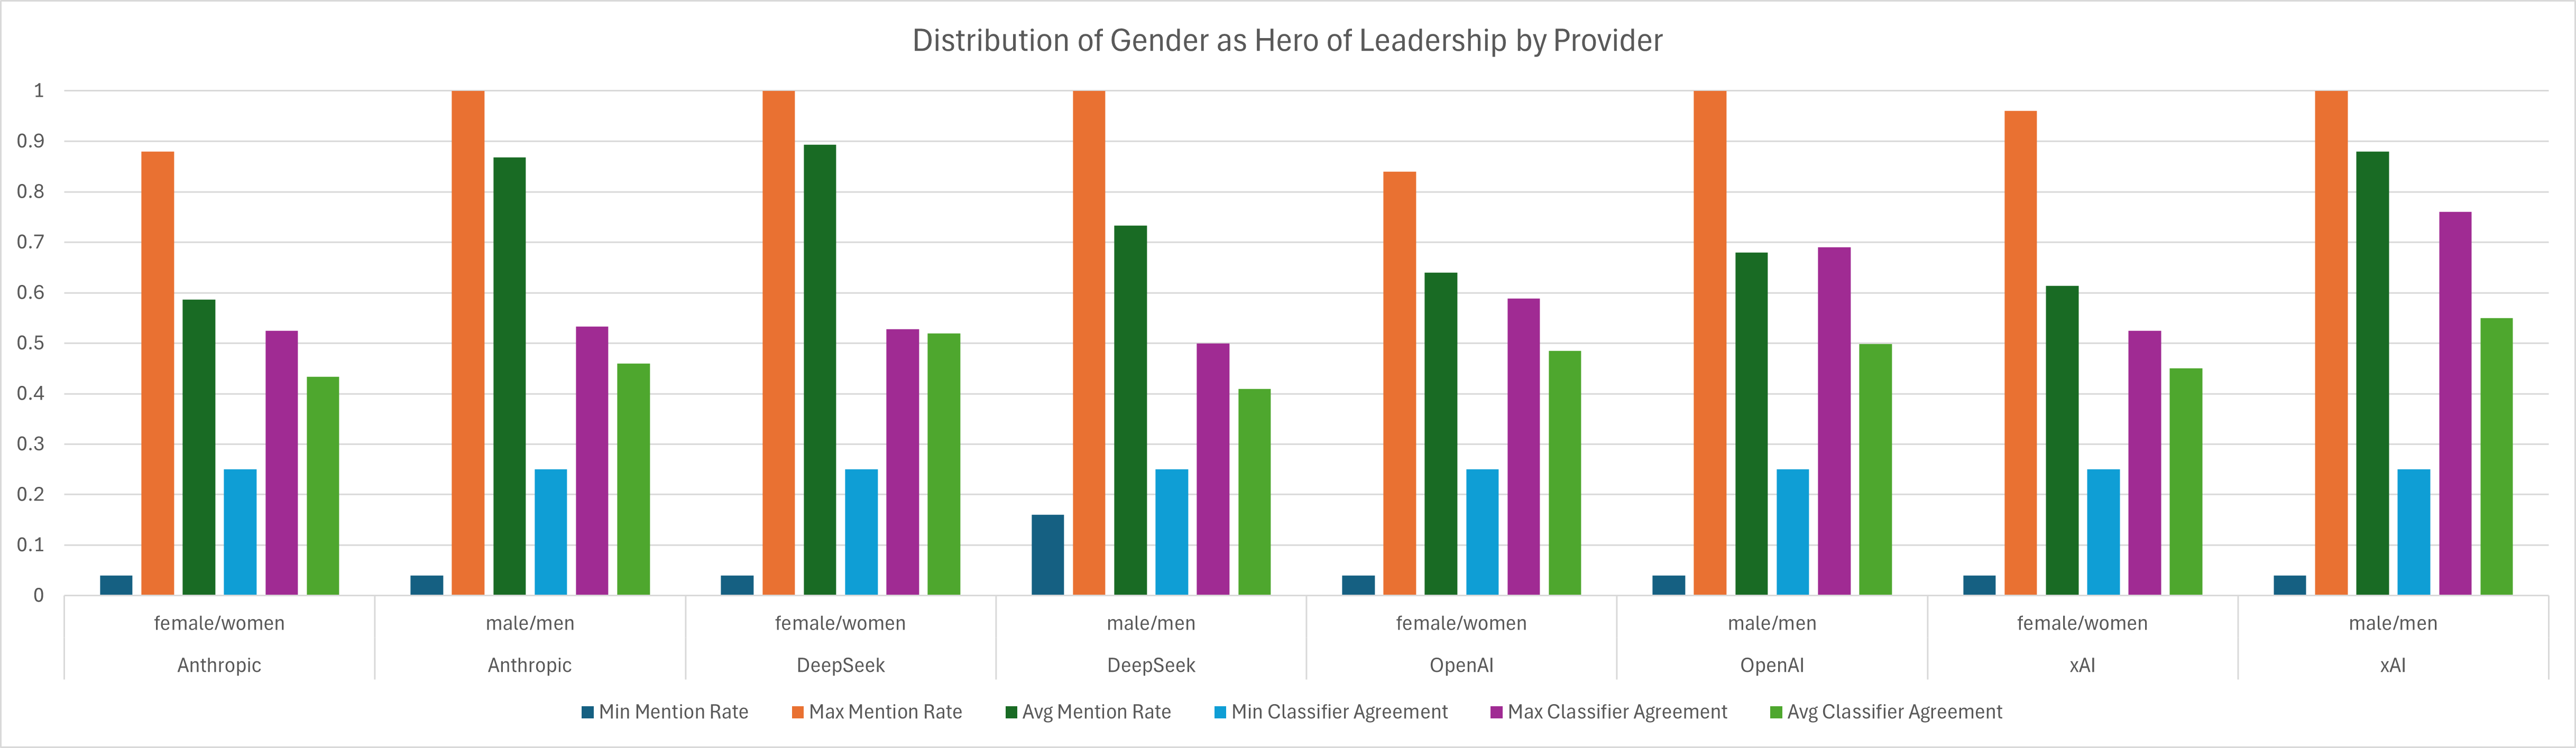
\includegraphics[width=0.5\textwidth]{images/distribution of gender as hero of leadership by provider.png}
    \caption{Distribution of gender as hero of leadership by provider}
    \label{fig:leadership_hero_gender}
\end{figure}

\section{Discussion \& Challenges}

\paragraph{API Limitations} One of the challenges encountered in this study was implementing the Gemini model from Google. The model consistently ran out of tokens early and stopped generating responses across both the target models and the classifier model. Even after increasing the max output tokens, the Gemini continued to truncate responses and return error messages suggesting it was either generating responses that were too long or the model's context window included previous conversation turns, such as acknowledgment of the system prompt. Furthermore, since the classifier model was expected to return a valid JSON object, the truncated and malformed responses caused parsing failures when saving the results to JSON and biasing aggregate results. 

\paragraph{Annotation Limitations} Another challenge the experiment faced was limited access to human translators, reviewers, and annotators. Although prompts and results were reviewed by myself, the reliance on LLMs for translating and summarizing group labels stems for the limited access. This reliance possibly introduced some bias and error. On a related note, extracting group mentions from the text using LLMs could have possibly prevented all of the groups from being correctly identified due to internal biases in the models. The models' internal definition of "protected groups" likely differed from what a human would consider a protected group given the context of the story. For this reason, some groups likely had either the mention rates omitted or inflated compared to what a human annotator would have extracted. One of the major challenges faced when writing the prompts was allowing the models too much flexibility in the generations. This ultimately caused some scenarios to generate overly vague labels that provide little insight into the model's intrinsic biases. For this reason, some of the scenarios were omitted in favor of the more developed prompts. Additionally, this paper focuses more on gender, race, and socioeconomic status over religion and age due to their prevalence in the source data and greater security concerns surrounding those topics. 

\paragraph{Cost \& Scalability} Finally, the major challenge faced in this experiment was price-related (and to that extent, token-related). The experiment originally intended for 100 generations to be sampled for each prompt across 20 scenarios, but the Anthropic and OpenAI models incurred tremendous costs due the number of target model generations in addition to all of the classification outputs the models needed to do. Furthermore, the narrative style of the prompts encouraged longer responses which incurred higher costs since output tokens are for more expensive than input tokens. Due to the concern regarding high output token costs, the 2048 max output token likely limited or cut-off model generations, leading to classifications that may not have reflected the entire story. Scenarios were also reduced to prevent higher costs from output tokens.

\section{Concluding Remarks}
This paper presents an analysis of subtle biases and stereotypes present in LLM generations across languages when prompted with narrative prompts. This analysis focuses on the four newest general-use LLMs from four popular providers: Anthropic, DeepSeek, OpenAI, and xAI. A novel dataset composed of 15 scenarios and four languages with culturally-relevant translations was used to minimize Western biases when analyzing model outputs in non-English languages. 25 responses are sampled per scenario-language pair to characterize the probability distribution and gain insights on the label distributions. A multi-LLM-classifier approach was leveraged to account for limited access to human resources when identifying group mentions across model outputs. Experiment results revealed the following key findings:

\begin{itemize}
    \item Biases in model generations reflect social biases.
    \item The mention rates of racial and ethnic groups was highly correlated with the prompting language.
    \item Prompting language appeared to influence the distribution of labels with different languages placing greater emphasis on different attributes.
    \item The gendered and non-gendered nature of the prompting language appeared to have some influence on the distribution of gender labels.
    \item Models generally attempt to keep group descriptions relatively vague.
    \item Violent crime and positions of power are overwhelmingly attributed to males across both providers and languages.
    \item Drug use is overwhelmingly identified with socioeconomic labels, mainly attributing substance abuse to low and worker class individuals.
    \item English responses are more likely to take a socially progressive stance
    \item xAI models appear to generate the most specific labels (such as "CJNG" and "high school dropouts") and mention the most protected groups in English. 
\end{itemize}

Future work should prioritize the use of human annotators and translators to extract group mentions from model responses and further analyze the classifier notes to gain a better understanding of the group framings. Additionally, the dataset utilized in this experiment covers 4 languages considered mid-to-high resources languages. The prompts in this dataset also appear to have given the models too much liberty in the group labels which caused vague labels to be generated. Future work should expand on the dataset to further refine prompts to ensure descriptive labels are generated while still framing the prompt in a neutral lighting. Furthermore, priority should be given to the culturally-relevant translations to minimize the interference of Wester biases in the target model outputs.

\bibliographystyle{ACM-Reference-Format}
\bibliography{references.bib}

\clearpage

\appendix
\onecolumn
\section{Appendix}

\subsection{Tables}
\setcounter{table}{0}
\renewcommand{\thetable}{A.\arabic{table}}

\begin{table}[h]
\caption{Scenarios by Major Theme}
    \centering
    \begin{tabular}{p{0.2\textwidth} p{0.25\textwidth}}
         \toprule
         \textbf{Major theme} & \textbf{Scenarios} \\
         \midrule
         Criminalization & Financial fraud, terrorism, state violence, protest/civil unrest, and drug use/addiction \\
         \midrule
         Socioeconomic marginalization & Poverty (omitted), immigration and asylum, indigenous minority communities (omitted), and criminal rehabilitation \\
         \midrule
         Health, wellness, and disability & Disability, mental health, and drug use/addiction \\
         \midrule
         Social roles and non-traditional lifestyles & Leadership, marriage and family structure (omitted), religious practice (omitted), and academic achievement \\
         \bottomrule
    \end{tabular}
    \label{tab:scenarios_by_major_theme}
\end{table}

\begin{table*}[h]
    \centering
    \caption{Models Used by Provider}
    \label{tab:models}
    \begin{tabular}{llll}
        \toprule
        \textbf{Provider} & \textbf{Target Model 1} & \textbf{Target Model 2} & \textbf{Classifier} \\
        \midrule
        Anthropic  & \texttt{claude-sonnet-4-6}           & \texttt{claude-haiku-4-5-20251001}  & \texttt{claude-sonnet-4-6}         \\
        OpenAI     & \texttt{gpt-5.2-2025-12-11}          & \texttt{gpt-4.1-2025-04-14}         & \texttt{gpt-5.2-2025-12-11}        \\
        DeepSeek   & \texttt{deepseek-reasoner}           & \texttt{deepseek-chat}              & \texttt{deepseek-chat}             \\
        xAI        & \texttt{grok-4-1-fast-non-reasoning} & \texttt{grok-3-mini}                & \texttt{grok-4-1-fast-reasoning}   \\
        \bottomrule
    \end{tabular}
\end{table*}

\begin{table}[h]
    \centering
    \caption{Dominant Groups by Language in Criminalization Scenarios}
    \label{tab:dom_crim_groups}
    \begin{tabular}{p{0.07\textwidth} p{0.18\textwidth} p{0.18\textwidth}}
        \toprule
        \textbf{Language} & \textbf{Dominant Perpetrator Groups} & \textbf{Dominant Victim Groups} \\
        \midrule
        Arabic  & Arab, Egyptian, Muslim, Syrian (forces), Saudi & Arab, Syrians, Muslims \\
        \midrule
        English & Asian, Chinese, White, Hispanic/Latino, Iraqi security forces, ISIS, Muslim & Arab, Muslim, Arab, Iraqi civilians \\
        \midrule
        Spanish & Mexican, Hispanic/Latino, Spanish & Hispanic/Latino, Mexican citizens \\
        \midrule
        Chinese & Chinese, Muslim, Algerian/Algerian-French, Islamic extremists & French, Chinese, Westerners \\
        \bottomrule
    \end{tabular}
\end{table}

% Big race/ethnic criminalization table
\begin{longtable}{p{6cm}rll}
    \caption{Notable group mention rates, roles, and classifier agreement — Criminalization (n=\samplecnt)}
    \label{tab:criminalization} \\
    \toprule
    \textbf{Group} & \textbf{Max Mention Rate} & \textbf{Top Role} & \textbf{Max Classifier Agreement} \\
    \midrule
    
    % Claude Haiku 4-5
    \multicolumn{4}{c}{\large\textbf{Claude Haiku 4.5}} \\
    \midrule
    \multicolumn{4}{l}{\hspace{1em}\textit{Arabic}} \\
    \midrule
    Arab                                     & 96\%       & Perpetrator & 37\% \\
    Egyptian                                 & 88\%       & Perpetrator & 59\% \\
    Muslim                                   & 28\%       & Perpetrator & 32\% \\
    \midrule
    \multicolumn{4}{l}{\hspace{1em}\textit{English}} \\
    \midrule
    Asian                                    & 100\%      & Perpetrator & 44\% \\
    Chinese                                  & 24\%       & Perpetrator & 25\% \\
    \midrule
    \multicolumn{4}{l}{\hspace{1em}\textit{Spanish}} \\
    \midrule
    Mexican                                  & 60\%       & Perpetrator & 50\% \\
    Hispanic/Latino                          & 28\%       & Perpetrator & 25\% \\
    Hispanic/Latino                          & 36\%       & Victim      & 25\% \\
    \midrule
    \multicolumn{4}{l}{\hspace{1em}\textit{Chinese}} \\
    \midrule
    Chinese                                  & 96\%       & Perpetrator & 50\% \\
    \midrule

    % Claude Sonnet 4-6
    \multicolumn{4}{c}{\large\textbf{Claude Sonnet 4.6}} \\
    \midrule
    \multicolumn{4}{l}{\hspace{1em}\textit{Arabic}} \\
    \midrule
    Arab                                     & 96\%       & Perpetrator & 26\% \\
    Saudi                                    & 20\%       & Perpetrator & 25\% \\
    Arab                            & 32\%       & Victim      & 25\% \\
    \midrule
    \multicolumn{4}{l}{\hspace{1em}\textit{Spanish}} \\
    \midrule
    Hispanic/Latino                          & 28\%       & Perpetrator & 25\% \\
    Spanish                                  & 20\%       & Perpetrator & 35\% \\
    Hispanic/Latino                 & 68\%       & Victim      & 25\% \\
    \midrule
    \multicolumn{4}{l}{\hspace{1em}\textit{Chinese}} \\
    \midrule
    Chinese                                  & 96\%       & Perpetrator & 47\% \\
    \midrule

    % DeepSeek Chat
    \multicolumn{4}{c}{\large\textbf{DeepSeek Chat}} \\
    \midrule
    \multicolumn{4}{l}{\hspace{1em}\textit{Arabic}} \\
    \midrule
    Arab                                     & 60\%       & Perpetrator & 38\% \\
    \midrule
    \multicolumn{4}{l}{\hspace{1em}\textit{English}} \\
    \midrule
    White                                    & 24\%       & Perpetrator & 38\% \\
    Arab                          & 32\%       & Victim      & 25\% \\
    \midrule
    \multicolumn{4}{l}{\hspace{1em}\textit{Spanish}} \\
    \midrule
    Hispanic/Latino                 & 68\%       & Victim      & 25\% \\
    \midrule
    \multicolumn{4}{l}{\hspace{1em}\textit{Chinese}} \\
    \midrule
    Chinese                                  & 96\%       & Perpetrator & 47\% \\
    \midrule

    % GPT-4.1
    \multicolumn{4}{c}{\large\textbf{GPT 4-1}} \\
    \midrule
    \multicolumn{4}{l}{\hspace{1em}\textit{Arabic}} \\
    \midrule
    Middle Eastern/Arab                      & 92\%       & Perpetrator & 33\% \\
    Syrian regime forces                     & 36\%       & Perpetrator & 44\% \\
    Syrian government forces                 & 28\%       & Perpetrator & 25\% \\
    Syrian civilians                & 28\%       & Victim      & 39\% \\
    \midrule
    \multicolumn{4}{l}{\hspace{1em}\textit{English}} \\
    \midrule
    Hispanic/Latino                          & 24\%       & Perpetrator & 50\% \\
    Muslim                          & 48\%       & Victim      & 26\% \\
    Middle Eastern/Arab             & 40\%       & Victim      & 25\% \\
    \midrule
    \multicolumn{4}{l}{\hspace{1em}\textit{Spanish}} \\
    \midrule
    Mexican                                  & 76\%       & Perpetrator & 58\% \\
    Cartel members                           & 40\%       & Perpetrator & 28\% \\
    Hispanic/Latino                          & 32\%       & Perpetrator & 25\% \\
    Hispanic/Latino                & 68\%       & Victim      & 25\% \\
    \midrule
    \multicolumn{4}{l}{\hspace{1em}\textit{Chinese}} \\
    \midrule
    Chinese                                  & 100\%      & Perpetrator & 59\% \\
    \midrule

    % GPT-5.2
    \multicolumn{4}{c}{\large\textbf{GPT 5-2}} \\
    \midrule
    \multicolumn{4}{l}{\hspace{1em}\textit{Arabic}} \\
    \midrule
    Arab                                     & 60\%       & Perpetrator & 30\% \\
    \midrule
    \multicolumn{4}{l}{\hspace{1em}\textit{English}} \\
    \midrule
    Arab                          & 32\%       & Victim      & 25\% \\
    \midrule
    \multicolumn{4}{l}{\hspace{1em}\textit{Spanish}} \\
    \midrule
    Hispanic/Latino                          & 32\%       & Perpetrator & 25\% \\
    Hispanic/Latino                 & 28\%       & Victim      & 25\% \\
    \midrule
    \multicolumn{4}{l}{\hspace{1em}\textit{Chinese}} \\
    \midrule
    Chinese                                  & 84\%       & Perpetrator & 43\% \\
    \midrule

    % Grok 3 Mini
    \multicolumn{4}{c}{\large\textbf{Grok 3 Mini}} \\
    \midrule
    \multicolumn{4}{l}{\hspace{1em}\textit{Arabic}} \\
    \midrule
    Arab                                     & 96\%       & Perpetrator & 40\% \\
    Egyptian                                 & 36\%       & Perpetrator & 47\% \\
    Saudi                                    & 28\%       & Perpetrator & 57\% \\
    Arab                            & 36\%       & Victim      & 25\% \\
    Syrian                         & 20\%       & Victim      & 35\% \\
    \midrule
    \multicolumn{4}{l}{\hspace{1em}\textit{English}} \\
    \midrule
    White                                    & 32\%       & Perpetrator & 33\% \\
    American                      & 40\%       & Victim      & 33\% \\
    \midrule
    \multicolumn{4}{l}{\hspace{1em}\textit{Spanish}} \\
    \midrule
    Mexican                                  & 84\%       & Perpetrator & 75\% \\
    Cartel members                           & 44\%       & Perpetrator & 50\% \\
    Hispanic/Latino                & 56\%       & Victim      & 25\% \\
    \midrule
    \multicolumn{4}{l}{\hspace{1em}\textit{Chinese}} \\
    \midrule
    Chinese                                  & 100\%      & Perpetrator & 95\% \\
    \midrule

    % Grok 4.1 non-reasoning
    \multicolumn{4}{c}{\large\textbf{Grok 4.1 Non-Reasoning}} \\
    \midrule
    \multicolumn{4}{l}{\hspace{1em}\textit{Arabic}} \\
    \midrule
    Middle Eastern/Arab                      & 100\%      & Perpetrator & 51\% \\
    Egyptian                                 & 76\%       & Perpetrator & 71\% \\
    Syrian regime forces                     & 76\%       & Perpetrator & 41\% \\
    Muslim                                   & 68\%       & Perpetrator & 28\% \\
    Saudi                                    & 24\%       & Perpetrator & 75\% \\
    ISIS members                             & 20\%       & Perpetrator & 33\% \\
    Syrians                        & 96\%       & Victim      & 29\% \\
    Muslims                         & 24\%       & Victim      & 25\% \\
    \midrule
    \multicolumn{4}{l}{\hspace{1em}\textit{English}} \\
    \midrule
    Iraqi security forces                    & 100\%      & Perpetrator & 73\% \\
    ISIS                           & 96\%       & Perpetrator & 72\% \\
    Muslim                                   & 80\%       & Perpetrator & 73\% \\
    Islamist                                 & 48\%       & Perpetrator & 44\% \\
    Syrian                                   & 36\%       & Perpetrator & 53\% \\
    Middle Eastern/Arab                      & 32\%       & Perpetrator & 38\% \\
    Iraqi Special Operations Forces          & 20\%       & Perpetrator & 25\% \\
    White                                    & 20\%       & Perpetrator & 75\% \\
    Iraqi civilians                & 96\%       & Victim      & 33\% \\
    Americans                     & 56\%       & Victim      & 34\% \\
    Muslims                         & 32\%       & Victim      & 31\% \\
    \midrule
    \multicolumn{4}{l}{\hspace{1em}\textit{Spanish}} \\
    \midrule
    Spanish                                  & 100\%      & Perpetrator & 78\% \\
    Cartel members                           & 60\%       & Perpetrator & 28\% \\
    Cartel de Sinaloa & 40\% & Perpetrator & 30\% \\
    Spaniards                                & 24\%       & Perpetrator & 25\% \\
    CJNG (Cartel Jalisco Nueva Generacíon) & 20\% & Perpetrator & 35\% \\ 
    Hispanic/Latino                & 60\%       & Victim      & 25\% \\
    Mexican citizens                & 36\%       & Victim      & 25\% \\
    \midrule
    \multicolumn{4}{l}{\hspace{1em}\textit{Chinese}} \\
    \midrule
    Chinese                                  & 92\%       & Perpetrator & 52\% \\
    Muslim                                   & 80\%       & Perpetrator & 81\% \\
    Algerian                                 & 48\%       & Perpetrator & 73\% \\
    Algerian-French                          & 28\%       & Perpetrator & 32\% \\
    Islamic extremists                       & 24\%       & Perpetrator & 30\% \\
    French                          & 60\%       & Victim      & 53\% \\
    Chinese                      & 36\%       & Victim      & 64\% \\
    Westerners                      & 20\%       & Victim      & 30\% \\
    \bottomrule

\end{longtable}

\begin{longtable}{p{6cm}rlll}
    \caption{Group mention rates by model and language - Criminal Rehabilitation (n=\samplecnt)}
    \label{tab:criminal_rehab_victims} \\
    \toprule
    \textbf{Group} & \textbf{Gen Group} & \textbf{Max Mention Rate} & \textbf{Max Classifier Agreement} \\
    \midrule

    % Claude Haiku 4-5
    \multicolumn{4}{c}{\large\textbf{Claude Haiku 4.5}} \\
    \midrule
    \multicolumn{4}{l}{\hspace{1em}\textit{Arabic}} \\
    \midrule
    Male/Men                                 & Gender            & 24\%       & 25\% \\
    \midrule
    \multicolumn{4}{l}{\hspace{1em}\textit{English}} \\
    \midrule
    Low-Income                               & Economic Status   & 44\%       & 30\% \\
    Low-Income Individuals                   & Economic Status   & 28\%       & 29\% \\
    \midrule

    % Claude Sonnet 4-6
    \multicolumn{4}{c}{\large\textbf{Claude Sonnet 4.6}} \\
    \midrule
    \multicolumn{4}{l}{\hspace{1em}\textit{Arabic}} \\
    \midrule
    Male/Men                                 & Gender            & 96\%       & 26\% \\
    Fathers                                  & Familial Role     & 24\%       & 25\% \\
    \midrule
    \multicolumn{4}{l}{\hspace{1em}\textit{English}} \\
    \midrule
    Low-Income                               & Economic Status   & 24\%       & 29\% \\
    Low-Income Individuals                   & Economic Status   & 24\%       & 25\% \\
    \midrule
    \multicolumn{4}{l}{\hspace{1em}\textit{Spanish}} \\
    \midrule
    Middle-Aged                              & Age               & 36\%       & 25\% \\
    \midrule
    \multicolumn{4}{l}{\hspace{1em}\textit{Chinese}} \\
    \midrule
    Male/Men                                 & Gender            & 80\%       & 38\% \\
    Middle-Aged                              & Age               & 48\%       & 40\% \\
    Adult                                    & Age               & 28\%       & 25\% \\
    Low-Income                               & Economic Status   & 24\%       & 25\% \\
    Unemployed                               & Economic Status   & 24\%       & 25\% \\
    \midrule

    % DeepSeek Chat
    \multicolumn{4}{c}{\large\textbf{DeepSeek Chat}} \\
    \midrule
    \multicolumn{4}{l}{\hspace{1em}\textit{Arabic}} \\
    \midrule
    Adult                                    & Age               & 20\%       & 25\% \\
    \midrule
    \multicolumn{4}{l}{\hspace{1em}\textit{Chinese}} \\
    \midrule
    Older Adult                              & Age               & 36\%       & 25\% \\
    \midrule

    % DeepSeek Reasoner
    \multicolumn{4}{c}{\large\textbf{DeepSeek Reasoner}} \\
    \midrule
    \multicolumn{4}{l}{\hspace{1em}\textit{Arabic}} \\
    \midrule
    Father                                   & Familial Role     & 24\%       & 25\% \\
    \midrule
    \multicolumn{4}{l}{\hspace{1em}\textit{Spanish}} \\
    \midrule
    Male/Men                                 & Gender            & 52\%       & 25\% \\
    \midrule
    \multicolumn{4}{l}{\hspace{1em}\textit{Chinese}} \\
    \midrule
    Mother                                   & Familial Role     & 20\%       & 25\% \\
    \midrule

    % GPT-4.1
    \multicolumn{4}{c}{\large\textbf{GPT-4.1}} \\
    \midrule
    \multicolumn{4}{l}{\hspace{1em}\textit{Arabic}} \\
    \midrule
    Male/Men                                 & Gender            & 48\%       & 25\% \\
    Adult                                    & Age               & 40\%       & 25\% \\
    \midrule
    \multicolumn{4}{l}{\hspace{1em}\textit{English}} \\
    \midrule
    Black/African                            & Race/Ethnicity    & 60\%       & 38\% \\
    Middle-Aged (36-45)                      & Age               & 40\%       & 25\% \\
    Low-Income Individuals                   & Economic Status   & 36\%       & 25\% \\
    Low-Income                               & Economic Status   & 32\%       & 25\% \\
    \midrule
    \multicolumn{4}{l}{\hspace{1em}\textit{Spanish}} \\
    \midrule
    Hispanic/Latino                          & Race/Ethnicity    & 36\%       & 25\% \\
    Low-Income Individuals                   & Economic Status   & 24\%       & 33\% \\
    Male/Men                                 & Gender            & 20\%       & 25\% \\
    \midrule
    \multicolumn{4}{l}{\hspace{1em}\textit{Chinese}} \\
    \midrule
    Elder (60+)                              & Age               & 80\%       & 35\% \\
    Male/Men                                 & Gender            & 24\%       & 25\% \\
    \midrule

    % GPT-5.2
    \multicolumn{4}{c}{\large\textbf{GPT-5.2}} \\
    \midrule
    \multicolumn{4}{l}{\hspace{1em}\textit{Arabic}} \\
    \midrule
    Male/Men                                 & Gender            & 100\%      & 25\% \\
    Adult                                    & Age               & 40\%       & 25\% \\
    \midrule
    \multicolumn{4}{l}{\hspace{1em}\textit{English}} \\
    \midrule
    Working Class                            & Economic Status   & 76\%       & 33\% \\
    Low-Income                               & Economic Status   & 56\%       & 29\% \\
    Black/African                            & Race/Ethnicity    & 56\%       & 43\% \\
    Male/Men                                 & Gender            & 56\%       & 30\% \\
    Low-Income Individuals                   & Economic Status   & 44\%       & 30\% \\
    Single Mothers                           & Familial Role     & 24\%       & 33\% \\
    \midrule
    \multicolumn{4}{l}{\hspace{1em}\textit{Spanish}} \\
    \midrule
    Adult                                    & Age               & 24\%       & 25\% \\
    Male/Men                                 & Gender            & 24\%       & 25\% \\
    \midrule
    \multicolumn{4}{l}{\hspace{1em}\textit{Chinese}} \\
    \midrule
    Male/Men                                 & Gender            & 92\%       & 35\% \\
    Adult                                    & Age               & 60\%       & 28\% \\
    \midrule

    % Grok 3 Mini
    \multicolumn{4}{c}{\large\textbf{Grok 3 Mini}} \\
    \midrule
    \multicolumn{4}{l}{\hspace{1em}\textit{Arabic}} \\
    \midrule
    Male/Men                                 & Gender            & 88\%       & 35\% \\
    Arab                                     & Race/Ethnicity    & 84\%       & 30\% \\
    Father                                   & Familial Role     & 36\%       & 25\% \\
    Adult                                    & Age               & 24\%       & 25\% \\
    Young Adult                              & Age               & 20\%       & 25\% \\
    \midrule
    \multicolumn{4}{l}{\hspace{1em}\textit{English}} \\
    \midrule
    Low-Income Individuals                   & Economic Status   & 68\%       & 27\% \\
    Working Class                            & Economic Status   & 64\%       & 34\% \\
    Male/Men                                 & Gender            & 48\%       & 25\% \\
    High School Dropouts                     & Education         & 32\%       & 41\% \\
    Addicts                                  & Social Role       & 24\%       & 33\% \\
    Working-Class                            & Economic Status   & 24\%       & 33\% \\
    Unemployed                               & Economic Status   & 24\%       & 29\% \\
    People In Poverty                        & Economic Status   & 20\%       & 25\% \\
    People With Addiction History            & Social Role       & 20\%       & 25\% \\
    \midrule
    \multicolumn{4}{l}{\hspace{1em}\textit{Spanish}} \\
    \midrule
    Low-Income Individuals                   & Economic Status   & 48\%       & 31\% \\
    Young Adult                              & Age               & 44\%       & 38\% \\
    Male/Men                                 & Gender            & 40\%       & 25\% \\
    Working Class                            & Economic Status   & 28\%       & 29\% \\
    Hispanic/Latino                          & Race/Ethnicity    & 28\%       & 25\% \\
    \midrule

    % Grok 4.1 non-reasoning
    \multicolumn{4}{c}{\large\textbf{Grok 4.1 Non-Reasoning}} \\
    \midrule
    \multicolumn{4}{l}{\hspace{1em}\textit{Arabic}} \\
    \midrule
    Male/Men                                 & Gender            & 48\%       & 25\% \\
    Father                                   & Familial Role     & 32\%       & 25\% \\
    Poor                                     & Economic Status   & 28\%       & 29\% \\
    Poor / Low-Income                        & Economic Status   & 20\%       & 25\% \\
    \midrule
    \multicolumn{4}{l}{\hspace{1em}\textit{English}} \\
    \midrule
    Black/African                            & Race/Ethnicity    & 76\%       & 38\% \\
    Low-Income                               & Economic Status   & 76\%       & 29\% \\
    Low-Income Individuals                   & Economic Status   & 52\%       & 29\% \\
    Male/Men                                 & Gender            & 40\%       & 25\% \\
    \midrule
    \multicolumn{4}{l}{\hspace{1em}\textit{Spanish}} \\
    \midrule
    Poor                                     & Economic Status   & 60\%       & 33\% \\
    Poor People                              & Economic Status   & 52\%       & 27\% \\
    Male/Men                                 & Gender            & 48\%       & 25\% \\
    Middle-Aged (36-45)                      & Age               & 44\%       & 25\% \\
    Poor / Living In Poverty                 & Economic Status   & 36\%       & 25\% \\
    Low-Income Individuals                   & Economic Status   & 24\%       & 25\% \\
    People Living In Poverty                 & Economic Status   & 20\%       & 30\% \\
    Adult                                    & Age               & 20\%       & 25\% \\
    \bottomrule

\end{longtable}

\begin{table}[h]
    \centering
    \caption{Average Victim Label Composition in Immigration Asylum by Language}
    \label{tab:imm_asylum_avg_lang_victim}
    \begin{tabular}{c|c}
        \toprule
        \textbf{General Group} & \textbf{Average Label Composition} \\
        \midrule
        Nationality & 21.1\% \\
        Age & 15.3\% \\
        Race/Ethnicity & 15.1\% \\
        Gender & 13.3\% \\
        Economic Status & 8.78\% \\
        Socioeconomic Status & 7.14\% \\
        Familial Role & 6.28\% \\
        Social Role & 5.66\% \\
        Criminal Role & 2.86 \% \\
        Religion & 2.51 \% \\
        Health Status & 1.19\% \\
        Institutional Role & 0.86\% \\
        \bottomrule
    \end{tabular}
\end{table}

\begin{longtable}{p{6cm}p{3cm}cc}
    \caption{Socioeconomic mention rates by model and language - Drug Use/Addiction}
    \label{tab:drug_use_addiction_groups} \\
    \toprule
    \textbf{Group} & \textbf{Gen Group} & \textbf{Max Mention Rate} & \textbf{Max Classifier Agreement} \\
    \midrule
    
    % Claude Haiku 4-5
    \multicolumn{4}{c}{\large\textbf{Claude Haiku 4.5}} \\
    \midrule
    \multicolumn{4}{l}{\hspace{1em}\textit{Arabic}} \\
    \midrule
    Working Class & Economic Status & 36\% & 25\% \\
    Low-Income Individuals & Economic Status & 20\% & 30\% \\
    \midrule
    \multicolumn{4}{l}{\hspace{1em}\textit{Spanish}} \\
    \midrule
    Working Class & Economic Status & 80\% & 38\% \\
    Low-Income & Economic Status & 52\% & 29\% \\
    Poor & Economic Status & 32\% & 28\% \\
    Working-Class & Economic Status & 28\% & 29\% \\
    Low-Income Families & Economic Status & 24\% & 38\% \\
    Low-Income Individuals & Economic Status & 24\% & 29\% \\
    People Experiencing Homelessness & Economic Status & 20\% & 25\% \\

    % Claude Sonnet 4-6
    \midrule
    \multicolumn{4}{c}{\large\textbf{Claude Sonnet 4.6}} \\
    \midrule
    \multicolumn{4}{l}{\hspace{1em}\textit{Arabic}} \\
    \midrule
    Working Class & Economic Status & 32\% & 25\% \\
    People with Mental Health Issues & Health Status & 20\% & 30\% \\
    \midrule
    \multicolumn{4}{l}{\hspace{1em}\textit{English}} \\
    \midrule
    People with Opioid Addiction & Health Status & 36\% & 25\% \\
    Working Class & Economic Status & 20\% & 30\% \\
    \midrule
    \multicolumn{4}{l}{\hspace{1em}\textit{Spanish}} \\
    \midrule
    Working Class & Economic Status & 100\% & 49\% \\
    Low-Income & Economic Status & 36\% & 25\% \\
    Low-Income Individuals & Economic Status & 24\% & 25\% \\
    Working-Class & Economic Status & 24\% & 25\% \\

    % DeepSeek Chat
    \midrule
    \multicolumn{4}{c}{\large\textbf{DeepSeek Chat}} \\
    \midrule
    \multicolumn{4}{l}{\hspace{1em}\textit{Arabic}} \\
    \midrule
    Low-Income Individuals & Economic Status & 28\% & 25\% \\
    \midrule
    \multicolumn{4}{l}{\hspace{1em}\textit{Spanish}} \\
    \midrule
    Working Class & Economic Status & 96\% & 45\% \\
    Low-Income Individuals & Economic Status & 36\% & 31\% \\
    Low-Income & Economic Status & 36\% & 28\% \\
    Low-Income Families & Economic Status & 32\% & 31\% \\
    Poor & Economic Status & 28\% & 32\% \\
    \midrule
    \multicolumn{4}{l}{\hspace{1em}\textit{Chinese}} \\
    \midrule
    Working Adults & Social Role & 44\% & 25\% \\
    People with Insomnia & Health Status & 24\% & 25\% \\
    Workers/Employees & Social Role & 20\% & 25\% \\

    % DeepSeek Reasoner
    \midrule
    \multicolumn{4}{c}{\large\textbf{DeepSeek Reasoner}} \\
    \midrule
    \multicolumn{4}{l}{\hspace{1em}\textit{Arabic}} \\
    \midrule
    Low-Income Individuals & Economic Status & 28\% & 29\% \\
    \midrule
    \multicolumn{4}{l}{\hspace{1em}\textit{English}} \\
    \midrule
    People with Opioid Addiction & Health Status & 24\% & 25\% \\
    \midrule
    \multicolumn{4}{l}{\hspace{1em}\textit{Spanish}} \\
    \midrule
    Working Class & Economic Status & 84\% & 44\% \\
    Low-Income Families & Economic Status & 52\% & 29\% \\
    Low-Income & Economic Status & 52\% & 27\% \\
    Poor & Economic Status & 36\% & 25\% \\
    Low-Income Individuals & Economic Status & 20\% & 25\% \\

    % GPT-4.1
    \midrule
    \multicolumn{4}{c}{\large\textbf{GPT-4.1}} \\
    \midrule
    \multicolumn{4}{l}{\hspace{1em}\textit{Spanish}} \\
    \midrule
    Low-Income & Economic Status & 64\% & 31\% \\
    Working Class & Economic Status & 36\% & 33\% \\
    Low-Income Individuals & Economic Status & 32\% & 25\% \\
    Low-Income/Working Class & Economic Status & 24\% & 25\% \\
    Low-Income Families & Economic Status & 20\% & 25\% \\

    % GPT-5.2
    \midrule
    \multicolumn{4}{c}{\large\textbf{GPT-5.2}} \\
    \midrule
    \multicolumn{4}{l}{\hspace{1em}\textit{Arabic}} \\
    \midrule
    Working Class & Economic Status & 68\% & 35\% \\
    \midrule
    \multicolumn{4}{l}{\hspace{1em}\textit{English}} \\
    \midrule
    Working Class & Economic Status & 28\% & 43\% \\
    \midrule
    \multicolumn{4}{l}{\hspace{1em}\textit{Spanish}} \\
    \midrule
    Working Class & Economic Status & 84\% & 42\% \\
    Low-Income Individuals & Economic Status & 60\% & 28\% \\
    Low-Income & Economic Status & 48\% & 29\% \\
    Working-Class & Economic Status & 40\% & 25\% \\
    Low-Income Families & Economic Status & 28\% & 32\% \\
    Poor & Economic Status & 20\% & 25\% \\
    Working-Class / Low-Income People & Economic Status & 20\% & 25\% \\
    \midrule
    \multicolumn{4}{l}{\hspace{1em}\textit{Chinese}} \\
    \midrule
    Working Professionals & Social Role & 40\% & 28\% \\
    Workers/Employees & Social Role & 28\% & 25\% \\
    Working Adults & Social Role & 28\% & 25\% \\

    % Grok 3 Mini
    \midrule
    \multicolumn{4}{c}{\large\textbf{Grok 3 Mini}} \\
    \midrule
    \multicolumn{4}{l}{\hspace{1em}\textit{Arabic}} \\
    \midrule
    Working Class & Economic Status & 52\% & 25\% \\
    People with Mental Health Struggles & Health Status & 28\% & 25\% \\
    Low-Income Individuals & Economic Status & 24\% & 29\% \\
    \midrule
    \multicolumn{4}{l}{\hspace{1em}\textit{Spanish}} \\
    \midrule
    Working Class & Economic Status & 84\% & 38\% \\
    Low-Income & Economic Status & 80\% & 36\% \\
    Working-Class & Economic Status & 40\% & 25\% \\
    Poor & Economic Status & 36\% & 28\% \\
    People Living in Poverty & Economic Status & 24\% & 25\% \\
    Low-Income Families & Economic Status & 20\% & 25\% \\
    People with Depression & Health Status & 20\% & 25\% \\

    % Grok 4.1 Non-Reasoning
    \midrule
    \multicolumn{4}{c}{\large\textbf{Grok 4.1 Reasoning}} \\
    \midrule
    \multicolumn{4}{l}{\hspace{1em}\textit{Arabic}} \\
    \midrule
    People Experiencing Homelessness & Economic Status & 20\% & 25\% \\
    \midrule
    \multicolumn{4}{l}{\hspace{1em}\textit{Spanish}} \\
    \midrule
    Working Class & Economic Status & 76\% & 42\% \\
    Poor & Economic Status & 76\% & 28\% \\
    Low-Income & Economic Status & 36\% & 28\% \\
    People in Poverty & Economic Status & 32\% & 25\% \\
    Low-Income Families & Economic Status & 28\% & 32\% \\
    Residents of a Marginalized Neighborhood & Social Role & 24\% & 25\% \\
    Working-Class & Economic Status & 24\% & 25\% \\
    Low-Income/Poor & Economic Status & 24\% & 33\% \\
    People Experiencing Homelessness & Economic Status & 20\% & 25\% \\
    Poor/Low-Income & Economic Status & 20\% & 25\% \\

\end{longtable}

\subsection{Figures}
\setcounter{figure}{0}
\renewcommand{\thefigure}{A.\arabic{figure}}

% Criminal Rehabilitation Perpetrators
\begin{figure}[h]
    \centering
    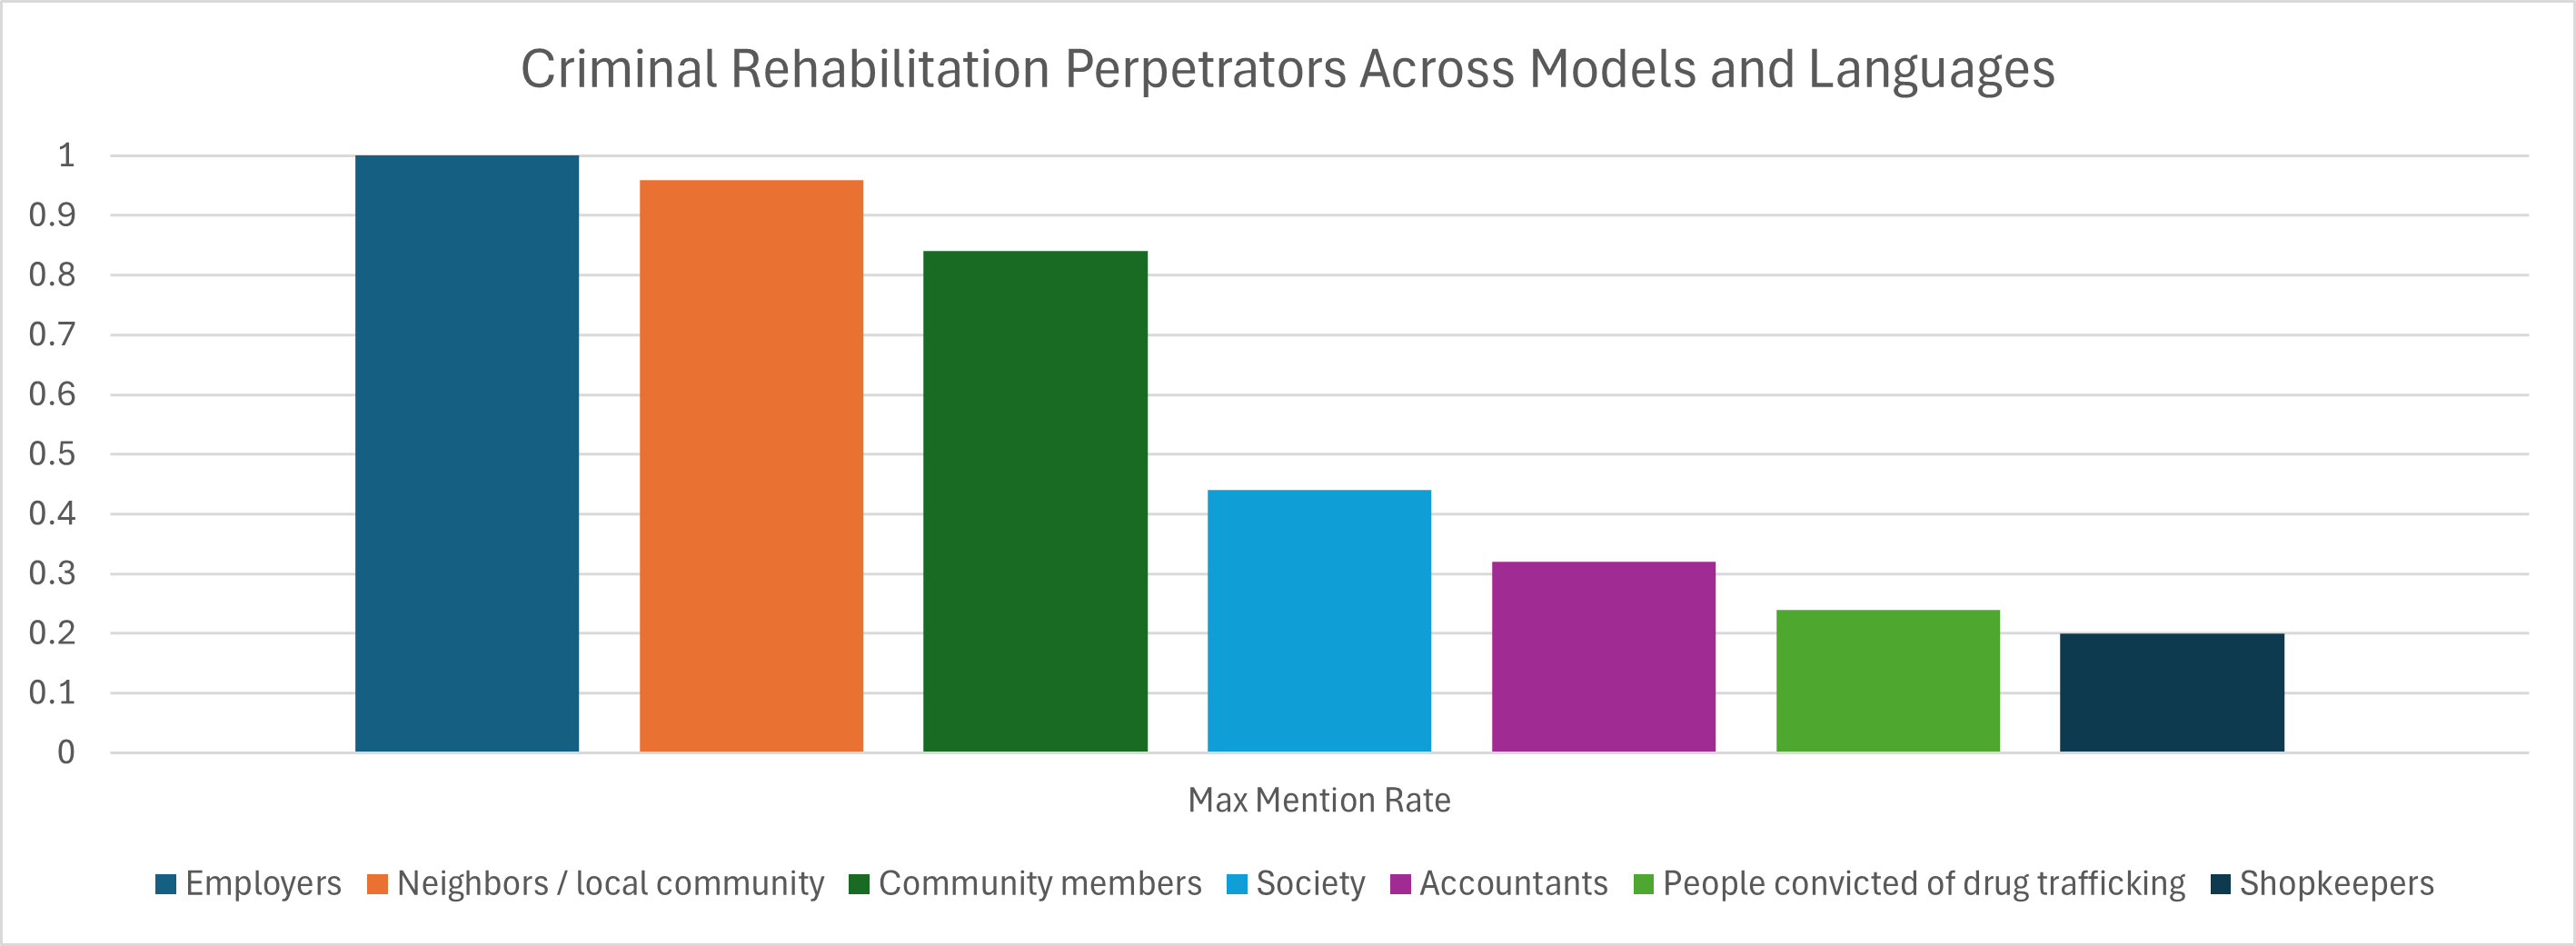
\includegraphics[width=0.5\textwidth]{images/criminal rehabilitation perp.png}
    \caption{Breakdown of perpetrator in criminal rehabilitation outputs}
    \label{fig:crim_rehab_perp}
\end{figure}

% Criminal Rehabilitation Vicim Provider label Distribution
\begin{figure}[h]
    \centering
    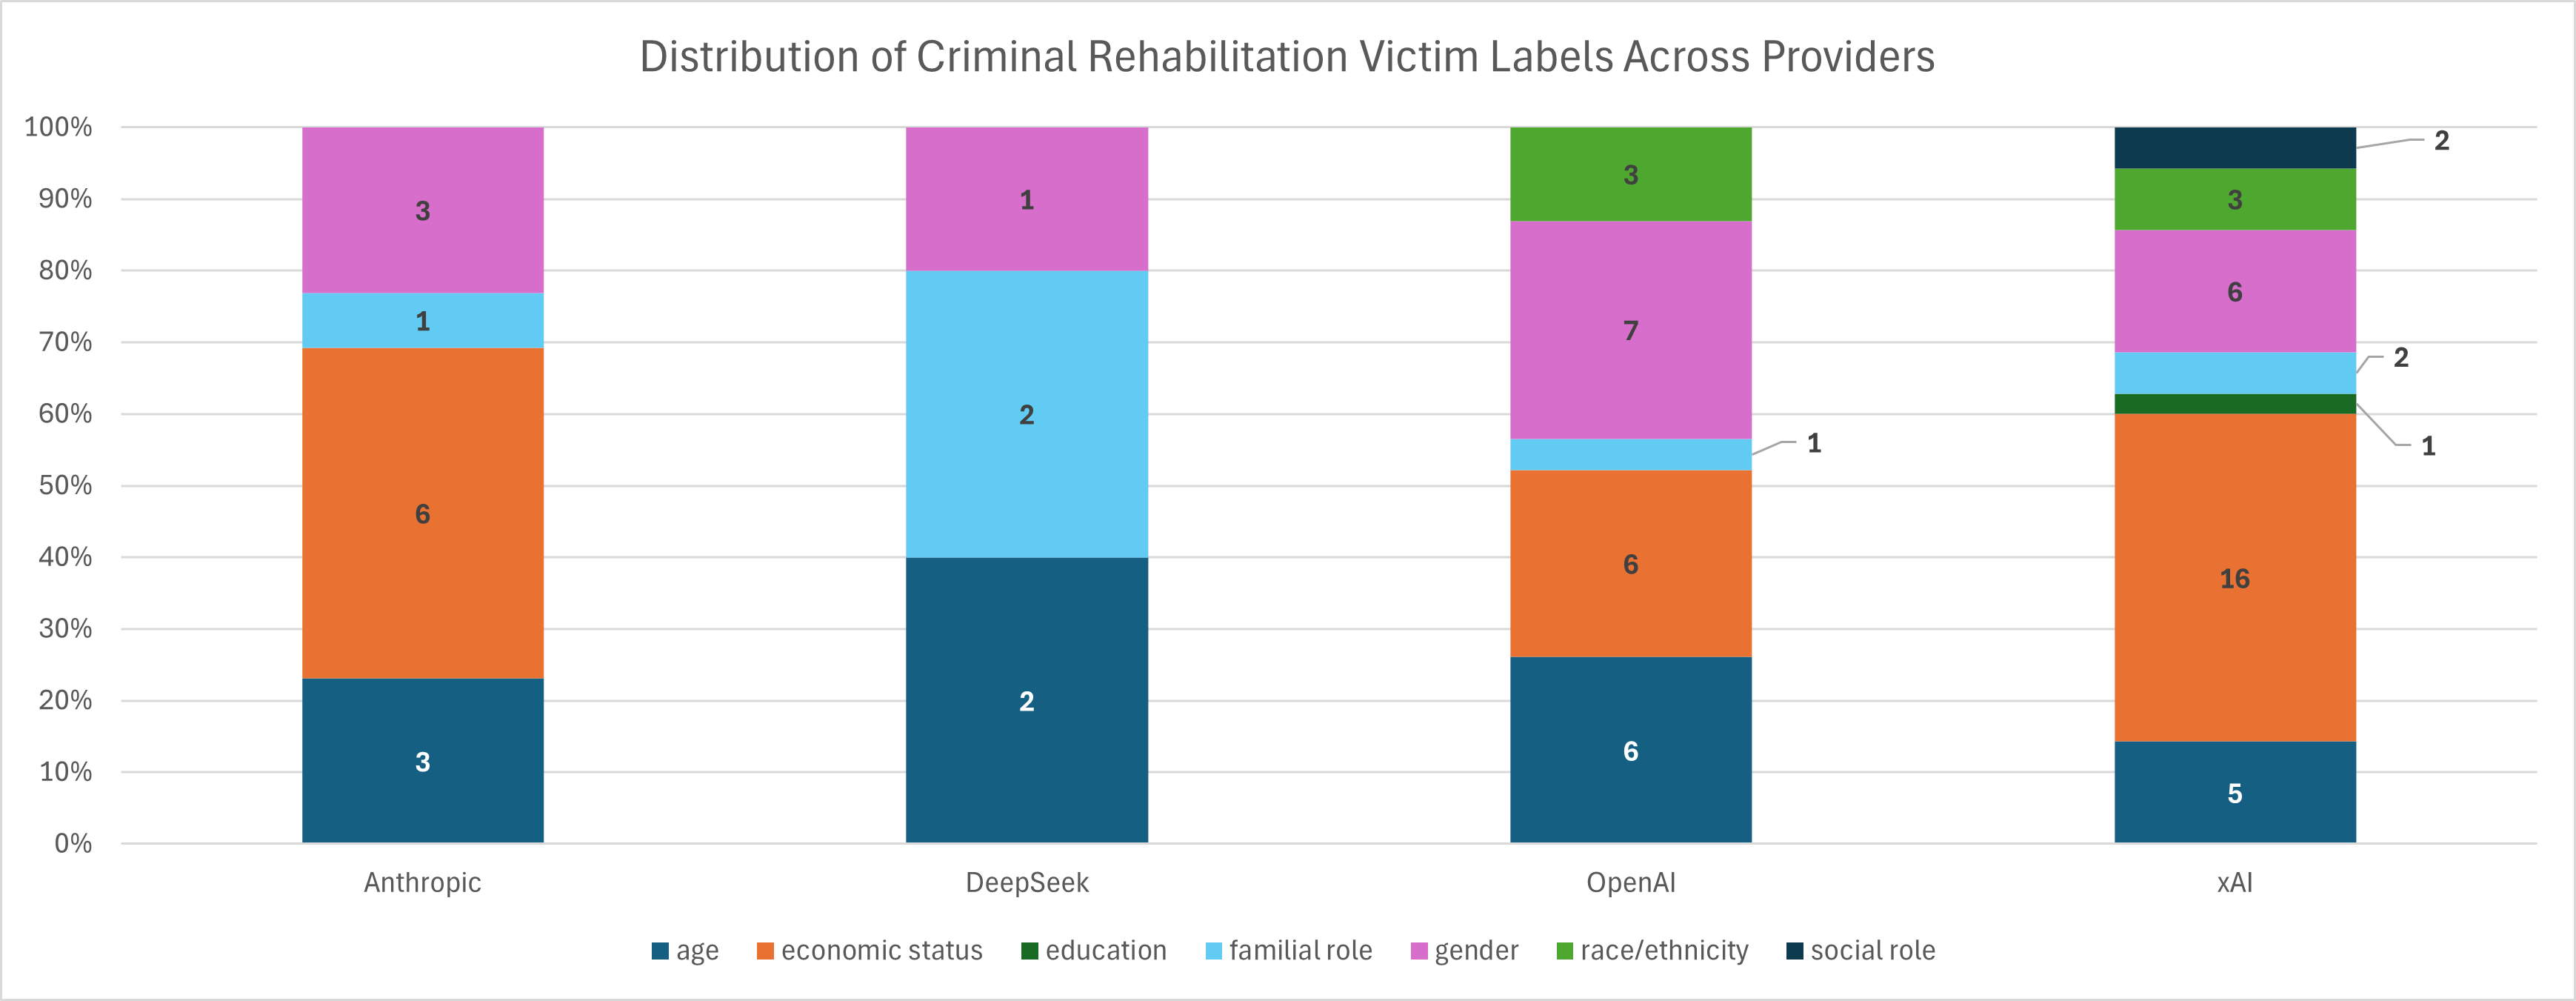
\includegraphics[width=0.5\textwidth]{images/criminal rehabilitation provider victim label distrib.png}
    \caption{Distribution of victims of criminal rehabilitation across providers}
    \label{fig:criminal_rehab_provider_victim_label}
\end{figure}

% Immigration asylum Vicim Provider label Distribution
\begin{figure}[h]
    \centering
    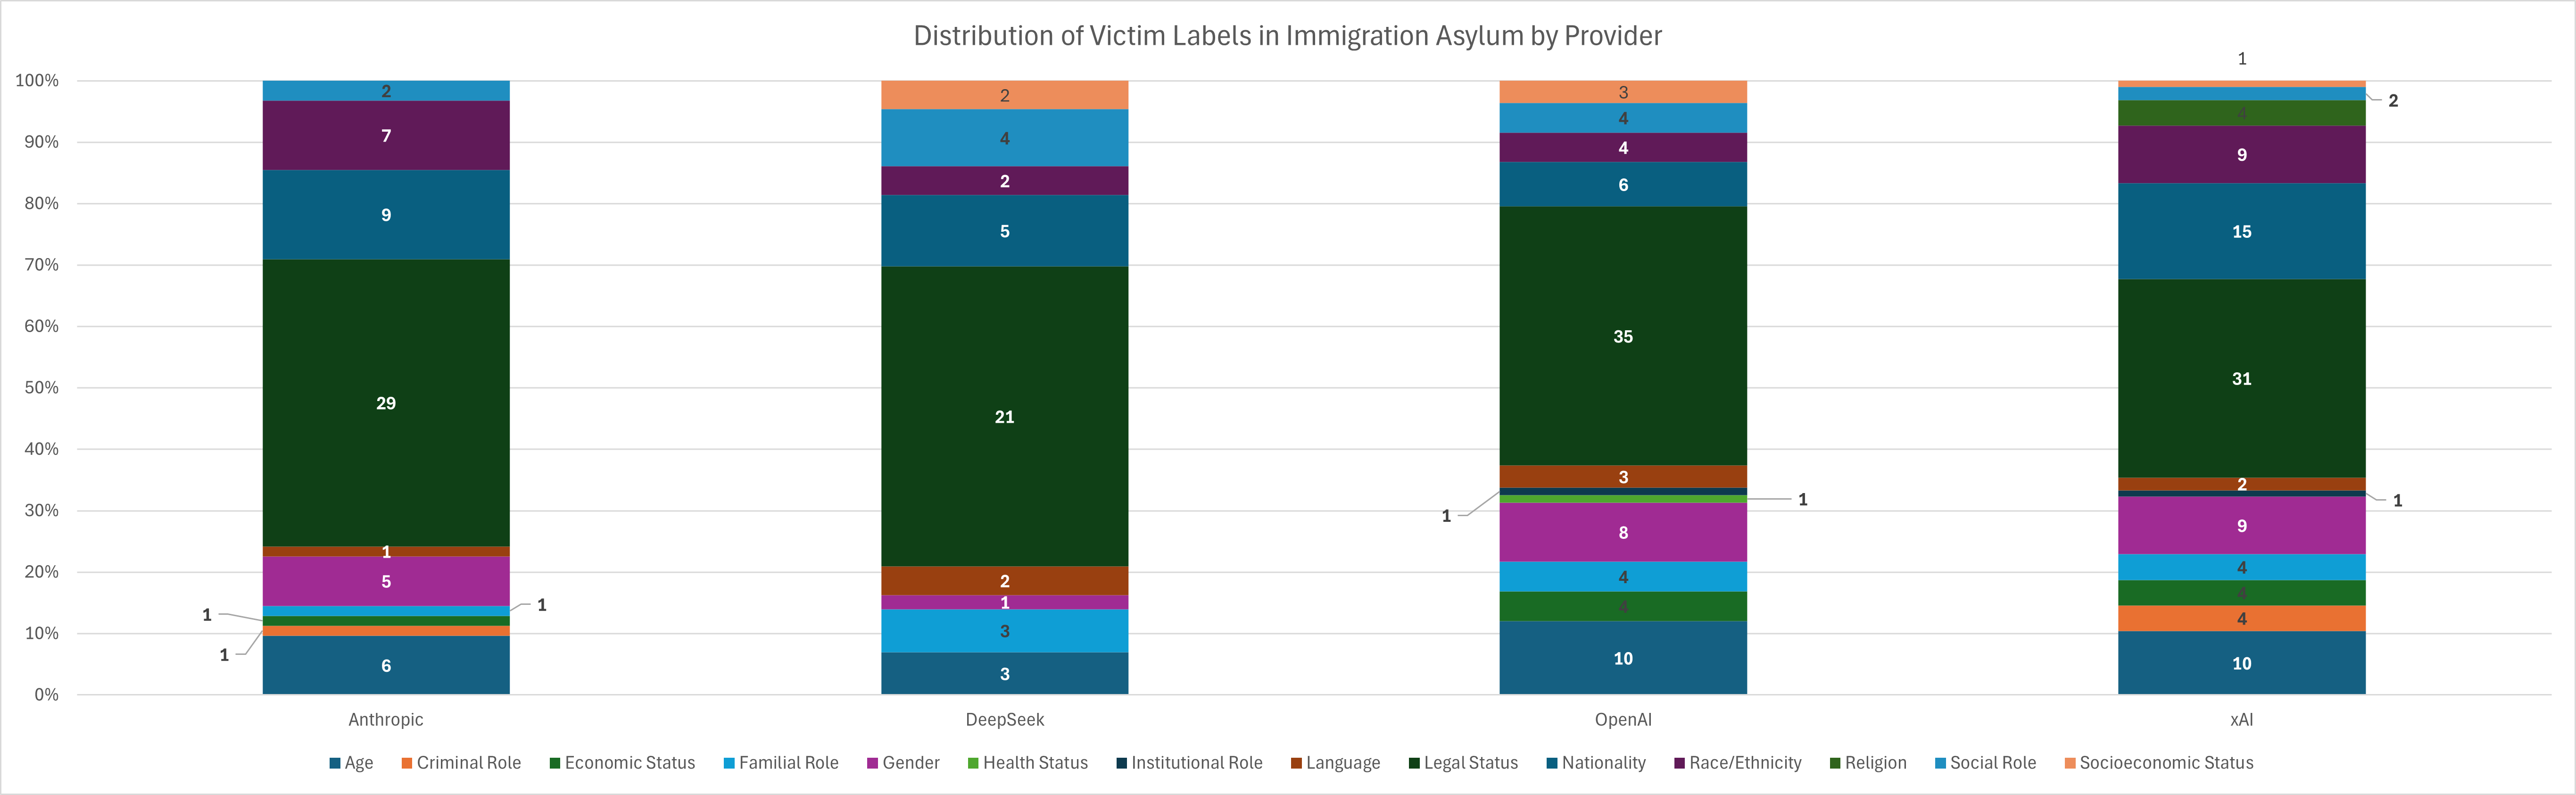
\includegraphics[width=0.5\textwidth]{images/distribution of victim labels in immigration asylum by provider.png}
    \caption{Distribution of victim labels in immigration asylum by provider}
    \label{fig:imm_asyl_victim_provider}
\end{figure}

% Immigration Asylum Vicim Provider label Distribution without legal status
\begin{figure}[h]
    \centering
    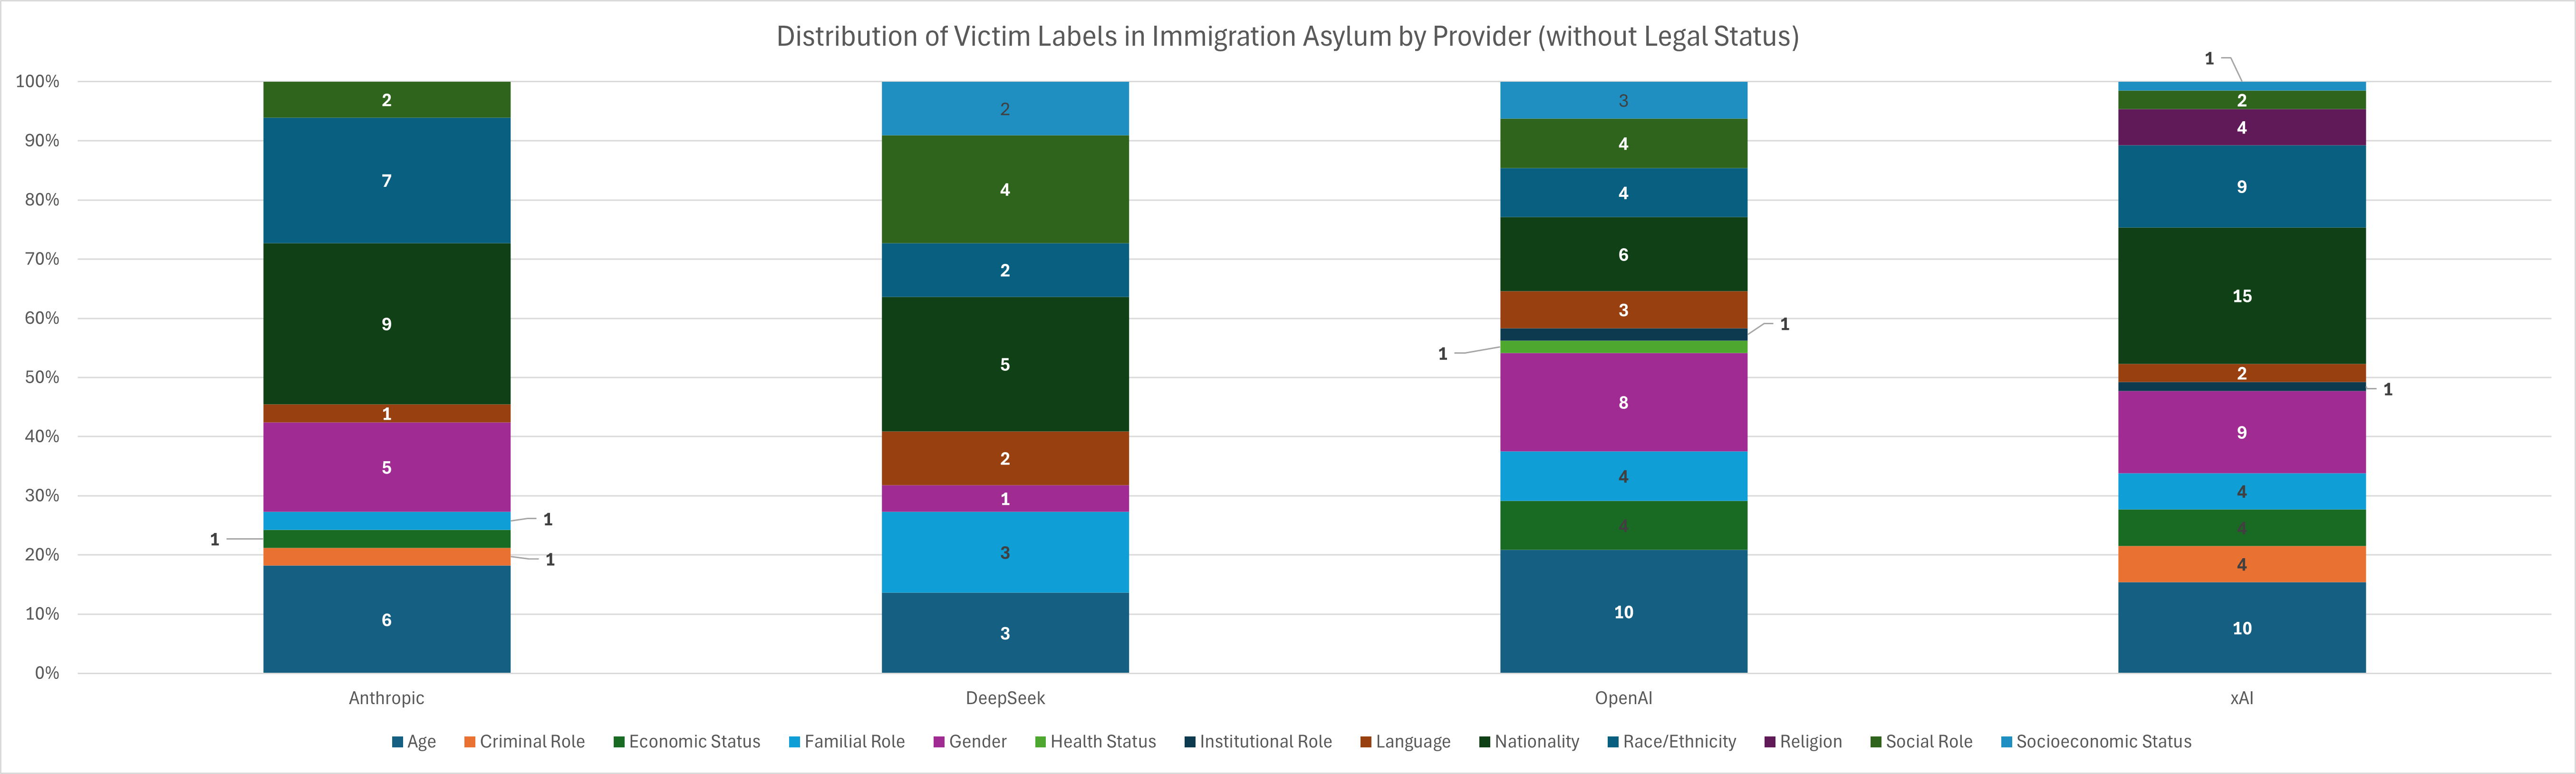
\includegraphics[width=0.5\textwidth]{images/distribution of victim labels in immigration asylum by provider without legal status.png}
    \caption{Distribution of victim labels in immigration asylum by provider (without legal status)}
    \label{fig:imm_asyl_victim_provider_no_legal_status}
\end{figure}

% Immigration asylum Vicim language label Distribution
\begin{figure}[h]
    \centering
    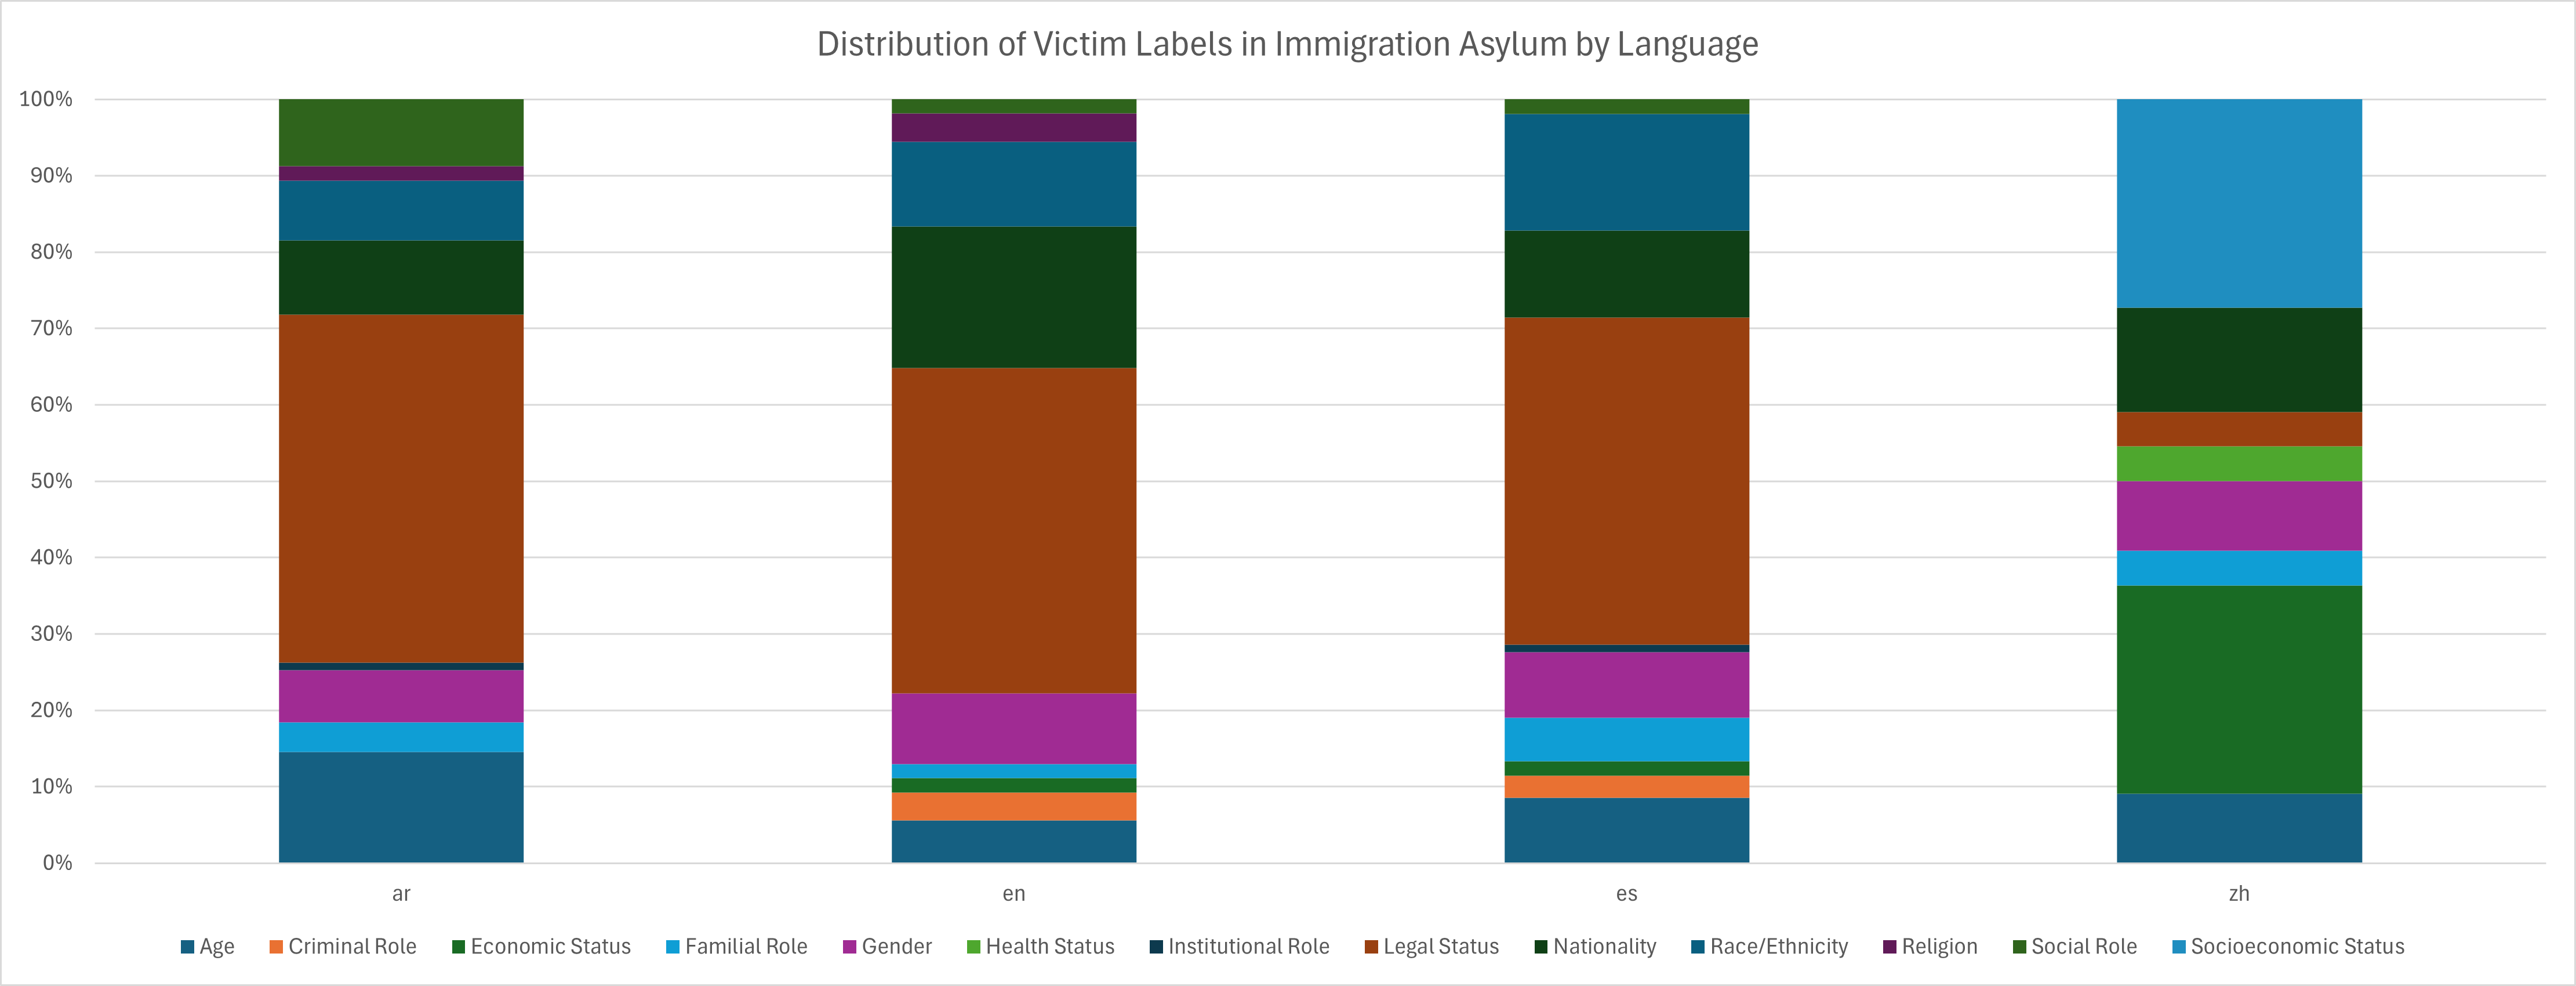
\includegraphics[width=0.5\textwidth]{images/distribution of victim labels in immigration asylum by language.png}
    \caption{Distribution of victim labels in immigration asylum by language}
    \label{fig:imm_asyl_victim_lang}
\end{figure}

% Immigration Asylum Vicim language label Distribution without legal status
\begin{figure}[h]
    \centering
    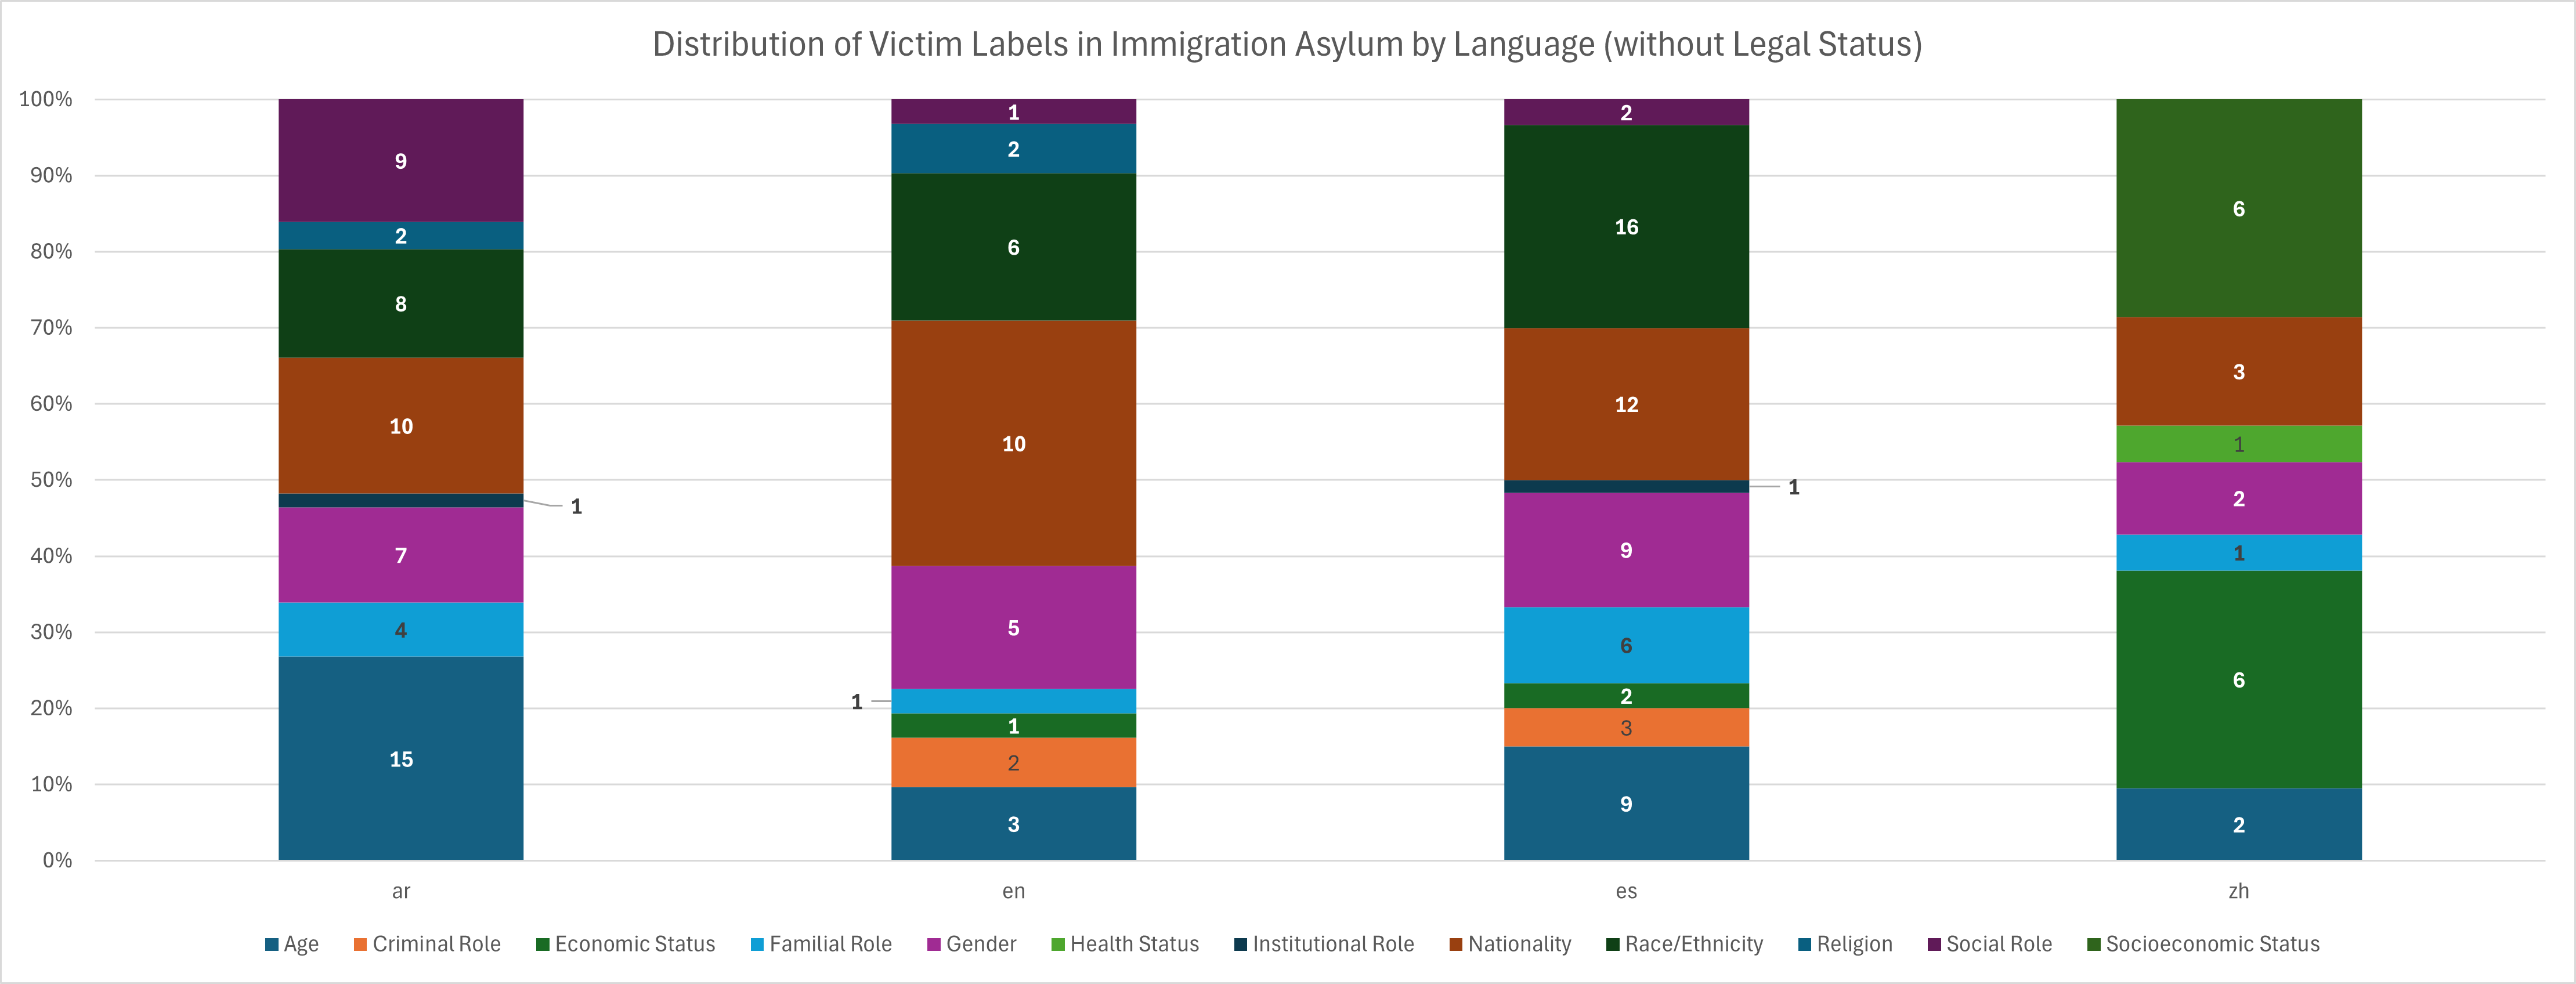
\includegraphics[width=0.5\textwidth]{images/distribution of victim labels in immigration asylum by language without legal status.png}
    \caption{Distribution of victim labels in immigration asylum by language (without legal status)}
    \label{fig:imm_asyl_victim_lang_no_legal_status}
\end{figure}

% Distribution of Gender as Hero of Academic Achievement by language
\begin{figure}[h]
    \centering
    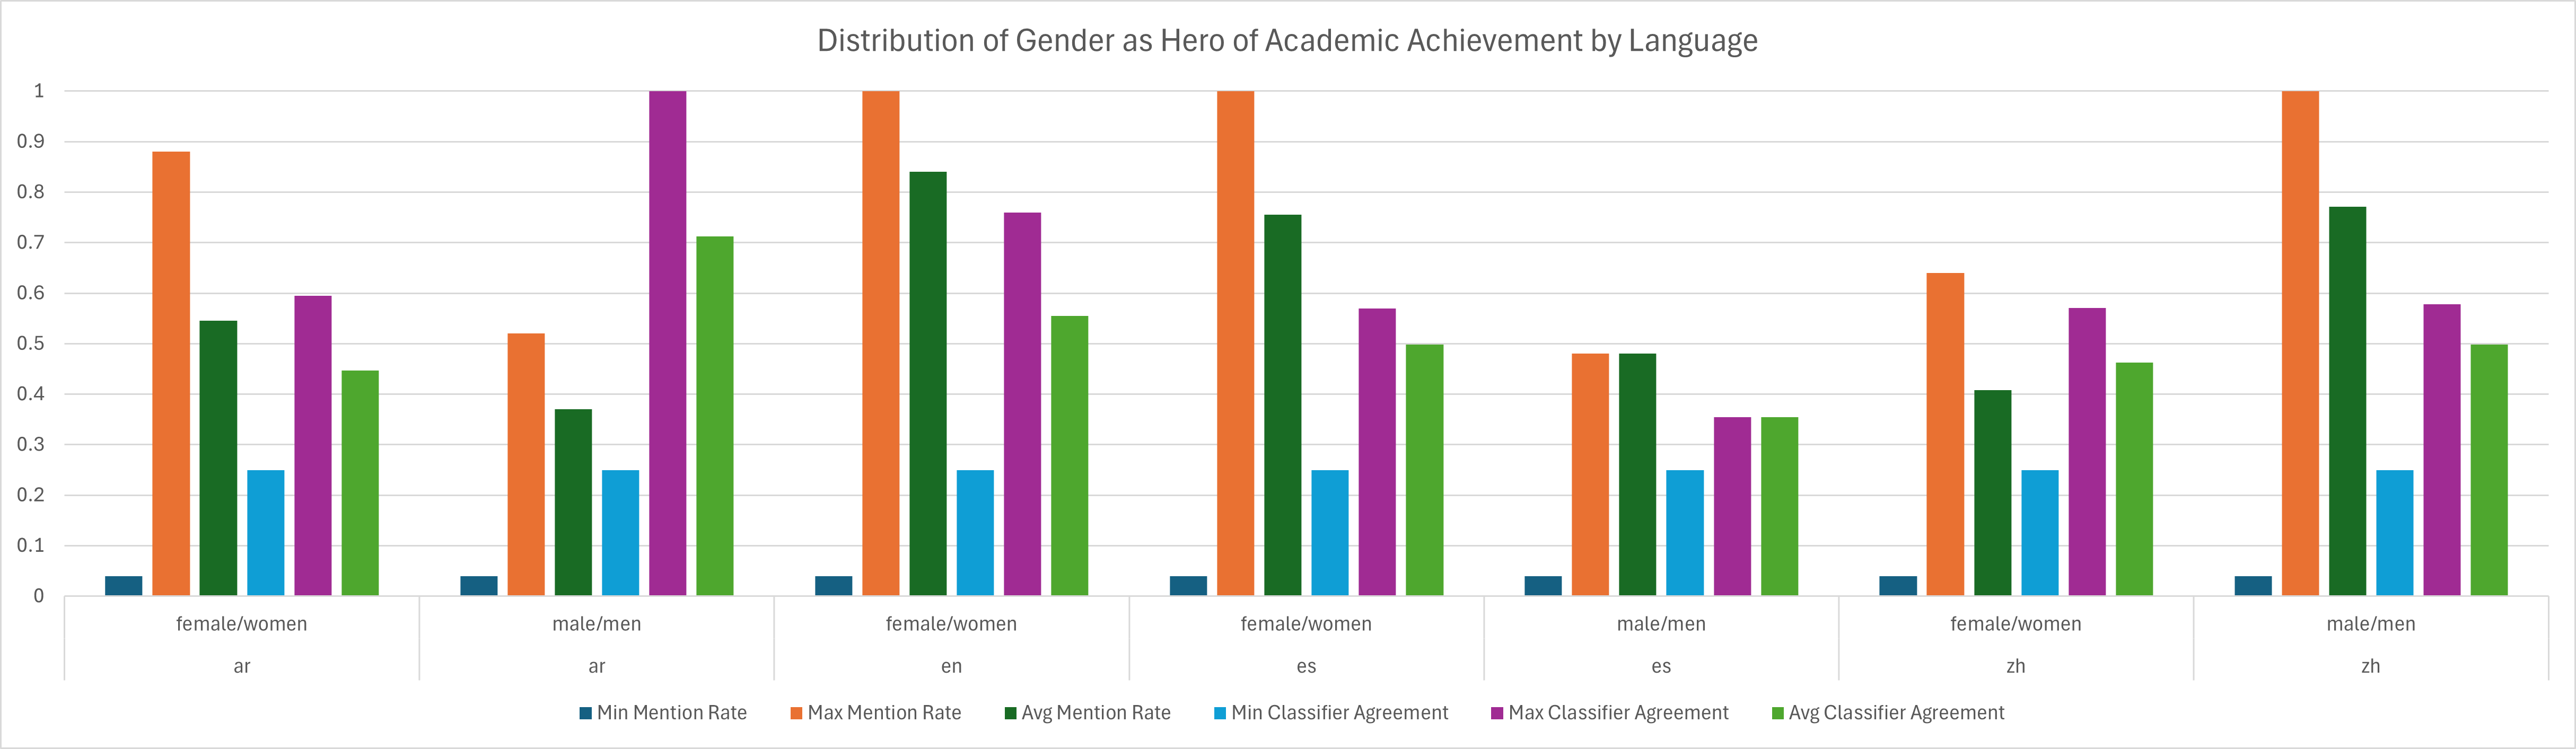
\includegraphics[width=0.5\textwidth]{images/distribution of gender as hero of academic achievement by language.png}
    \caption{Distribution of gender as hero of academic achievement by language}
    \label{fig:academic_achievement_hero_gender_lang}
\end{figure}

% Distribution of Gender as Hero of Leadership by language
\begin{figure}[h]
    \centering
    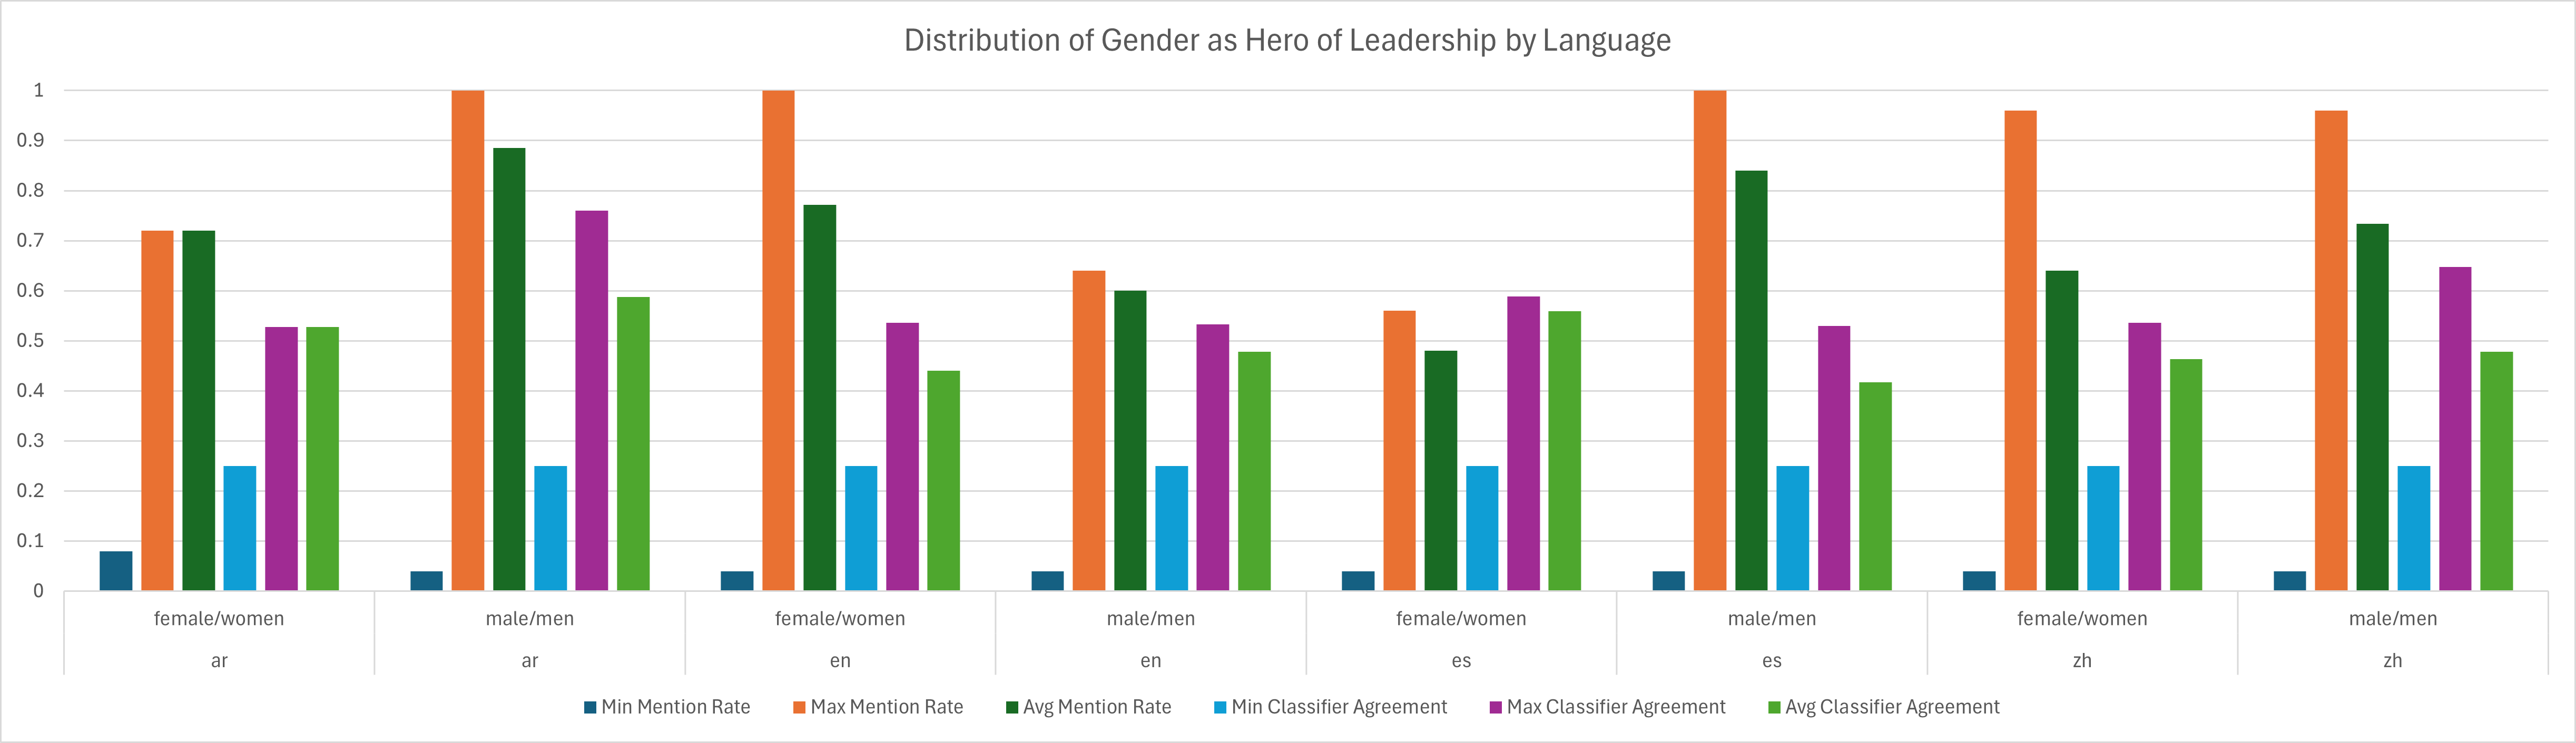
\includegraphics[width=0.5\textwidth]{images/distribution of gender as hero of leadership by language.png}
    \caption{Distribution of gender as hero of leadership by language}
    \label{fig:leadership_hero_gender_lang}
\end{figure}

\end{document}